\documentclass[11pt,a4paper,twocolumn]{article}

%------------------------------------------------------------------------------
%	REQUIRED PACKAGES AND  CONFIGURATIONS
%------------------------------------------------------------------------------
% PACKAGES FOR TITLES
\usepackage{titlesec}
\usepackage{color}

% PACKAGES FOR LANGUAGE AND FONT
\usepackage[utf8]{inputenc}
\usepackage[english]{babel}
\usepackage[T1]{fontenc} % Font encoding

% PACKAGES FOR IMAGES
\usepackage{graphicx}
\graphicspath{{Images/}} % Path for images' folder
\usepackage{eso-pic} % For the background picture on the title page
\usepackage{subfig} % Numbered and caption subfigures using \subfloat
\usepackage{caption} % Coloured captions
\usepackage{transparent}

\usepackage{tikz}
\usetikzlibrary{
    patterns,
    overlay-beamer-styles,
    datavisualization,
    datavisualization.formats.functions,
    fit,
    trees,
    backgrounds,
    mindmap,
    positioning,
    shapes.geometric,
    arrows
}

\usepackage{pgfplots}  
\usepgfplotslibrary{
    groupplots,
    units
}

\usepackage{tabularx}
\usepackage{longtable} % Tables that can span several pages
\usepackage{colortbl}

% STANDARD MATH PACKAGES
\usepackage{amsmath}
\usepackage{amsthm}
\usepackage{amsfonts}
\usepackage{bm}
\usepackage[overload]{empheq}  % For braced-style systems of equations

% PACKAGES FOR TABLES
\usepackage{tabularx}
\usepackage{longtable} % tables that can span several pages
\usepackage{colortbl}

% PACKAGES FOR ALGORITHMS (PSEUDO-CODE)
\usepackage{algorithm}
\usepackage{algorithmic}

% PACKAGES FOR REFERENCES & BIBLIOGRAPHY
\usepackage[colorlinks=true,linkcolor=black,anchorcolor=black,citecolor=black,filecolor=black,menucolor=black,runcolor=black,urlcolor=black]{hyperref} % Adds clickable links at references
\usepackage{cleveref}
\usepackage[square, numbers, sort&compress]{natbib} % Square brackets, citing references with numbers, citations sorted by appearance in the text and compressed
% \bibliographystyle{plain} % You may use a different style adapted to your field

% PACKAGES FOR THE APPENDIX
\usepackage{appendix}

% PACKAGES FOR ITEMIZE & ENUMERATES 
\usepackage{enumitem}

% OTHER PACKAGES
\usepackage{amsthm,thmtools,xcolor} % Coloured "Theorem"
\usepackage{comment} % Comment part of code
\usepackage{fancyhdr} % Fancy headers and footers
\usepackage{lipsum} % Insert dummy text
\usepackage{tcolorbox} % Create coloured boxes (e.g. the one for the key-words)
\usepackage{stfloats} % Correct position of the tables

%-------------------------------------------------------------------------
%	NEW COMMANDS DEFINED
%-------------------------------------------------------------------------
% EXAMPLES OF NEW COMMANDS -> here you see how to define new commands
\newcommand{\bea}{\begin{eqnarray}} % Shortcut for equation arrays
\newcommand{\eea}{\end{eqnarray}}
\newcommand{\e}[1]{\times 10^{#1}}  % Powers of 10 notation
\newcommand{\mathbbm}[1]{\text{\usefont{U}{bbm}{m}{n}#1}} % From mathbbm.sty
\newcommand{\pdev}[2]{\frac{\partial#1}{\partial#2}}
\newcommand\width{0.35}
\newcommand\widthPCA{0.4}

% Set the geometric layout of the document
\usepackage{geometry}
\geometry{
  top=3cm,
  left = 2.0cm,
  right = 2.0cm,
  bottom=2cm,
  headheight= 2cm,
  headsep= 0cm,
}
\raggedbottom 

% Create color bluePoli (-> manuale grafica coordinata:  https://www.polimi.it/fileadmin/user_upload/il_Politecnico/grafica-coordinata/2015_05_11_46xy_manuale_grafica_coordinata.pdf)
\definecolor{bluePoli}{cmyk}{0.4,0.1,0,0.4}

% Custom theorem environments
\declaretheoremstyle[
  headfont=\color{bluePoli}\normalfont\bfseries,
  bodyfont=\color{black}\normalfont\itshape,
]{colored}

\captionsetup[figure]{labelfont={color=bluePoli}} % Set colour of the captions
\captionsetup[table]{labelfont={color=bluePoli}} % Set colour of the captions
\captionsetup[algorithm]{labelfont={color=bluePoli}} % Set colour of the captions

\theoremstyle{colored}
\newtheorem{theorem}{Theorem}[section]
\newtheorem{proposition}{Proposition}[section]

% Enhances the features of the standard "table" and "tabular" environments.
\newcommand\T{\rule{0pt}{2.6ex}}
\newcommand\B{\rule[-1.2ex]{0pt}{0pt}}

% Algorithm description
\newcounter{algsubstate}
\renewcommand{\thealgsubstate}{\alph{algsubstate}}
\newenvironment{algsubstates}{
    \setcounter{algsubstate}{0}%
    \renewcommand{\STATE}{%
    \stepcounter{algsubstate}%
    \Statex {\small\thealgsubstate:}\space}
    }{}
    
% Custom theorem environment
\newcolumntype{L}[1]{>{\raggedright\let\newline\\\arraybackslash\hspace{0pt}}m{#1}}
\newcolumntype{C}[1]{>{\centering\let\newline\\\arraybackslash\hspace{0pt}}m{#1}}
\newcolumntype{R}[1]{>{\raggedleft\let\newline\\\arraybackslash\hspace{0pt}}m{#1}}

% Custom itemize environment
\setlist[itemize,1]{label=$\bullet$}
\setlist[itemize,2]{label=$\circ$}
\setlist[itemize,3]{label=$-$}
\setlist{nosep}

% Set separation of columns 
\setlength{\columnsep}{30pt}

% Create command for background pic
\newcommand\BackgroundPic{% Adding background picture
	\put(230,358){
		\parbox[b][\paperheight]{\paperwidth}{%
			\vfill
			\centering
			\transparent{0.4}
			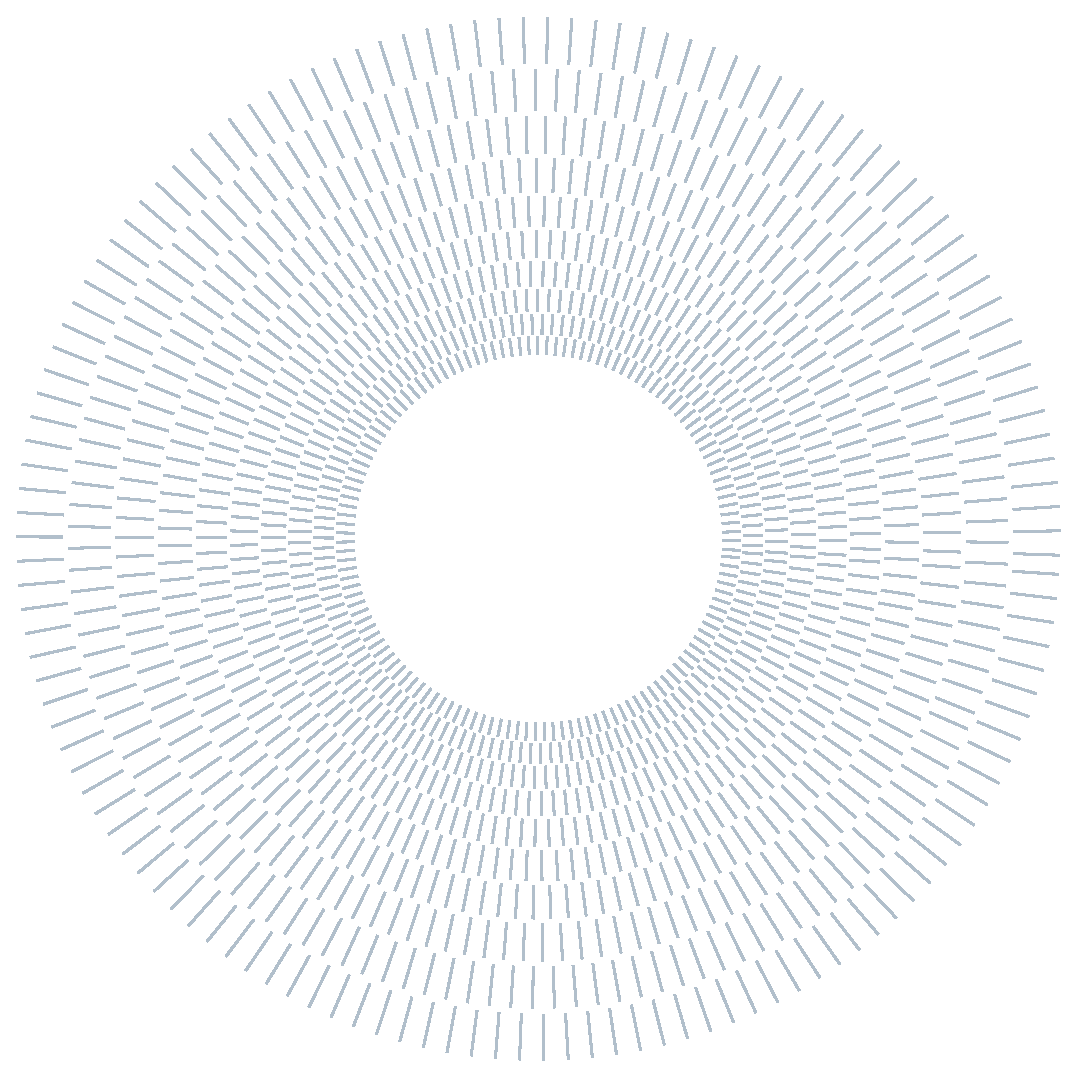
\includegraphics[width=0.5\paperwidth]{raggiera_polimi.eps}%
			\vfill
}}}

% Set indentation
\setlength\parindent{0pt}

% Custom title commands
\titleformat{\section}
{\color{bluePoli}\normalfont\Large\bfseries}
{\color{bluePoli}\thesection.}{1em}{}
\titlespacing*{\section}
{0pt}{2ex}{1ex}

\titleformat{\subsection}
{\color{bluePoli}\normalfont\large\bfseries}
{\color{bluePoli}\thesubsection.}{1em}{}
\titlespacing*{\subsection}
{0pt}{2ex}{1ex}

% Custom headers and footers
\pagestyle{fancy}
\fancyhf{}
      
\fancyfoot{}
\fancyfoot[C]{\thepage} % page
\renewcommand{\headrulewidth}{0mm} % headrule width
\renewcommand{\footrulewidth}{0mm} % footrule width

\makeatletter
\patchcmd{\headrule}{\hrule}{\color{black}\hrule}{}{} % headrule
\patchcmd{\footrule}{\hrule}{\color{black}\hrule}{}{} % footrule
\makeatother

% -> Create the header
\chead[C]{
\centering
\begin{tcolorbox}[arc=0pt, boxrule=0pt, colback=bluePoli!60, width=\textwidth, colupper=white]
    \textbf{Executive summary} \hfill \textbf{\author}  
\end{tcolorbox}
}

% Insert here the info that will be displayed into your Title page 
% -> title of your work
\renewcommand{\title}{Data Driven Approach to Turbomachinery Blade Design}
% -> author name and surname
\renewcommand{\author}{Antonio Pucciarelli}
% -> MSc course
\newcommand{\course}{Aeronautical Engineering - Ingegneria Aeronautica}
% -> advisor name and surname
\newcommand{\advisor}{Prof. Sergio Lavagnoli} % insert if any otherwise comment
% IF AND ONLY IF you need to modify the co-supervisors you also have to modify the file Configuration_files/title_page.tex (ONLY where it is marked)
\newcommand{\promoter}{Prof. Paolo Gaetani}
%\newcommand{\secondcoadvisor}{Name Surname} % insert if any otherwise comment
% -> academic year
\newcommand{\YEAR}{2022-2023}

%-------------------------------------------------------------------------
%	BEGIN OF YOUR DOCUMENT
%-------------------------------------------------------------------------
\begin{document}

%-----------------------------------------------------------------------------
% TITLE PAGE
%-----------------------------------------------------------------------------
% Do not change Configuration_files/TitlePage.tex (Modify it IF AND ONLY IF you need to add or delete the Co-advisors)
% This file creates the Title Page of the document
% DO NOT REMOVE SPACES BETWEEN LINES!

\twocolumn[{\begin{@twocolumnfalse}

\AddToShipoutPicture*{\BackgroundPic}

\hspace{-0.6cm}
\includegraphics[width=0.6\textwidth]{logo_polimi_ing_indinf.eps}

\vspace{-1mm}
\fontsize{0.3cm}{0.5cm}\selectfont \bfseries \textsc{\color{bluePoli} Executive Summary of the Thesis}\\

\vspace{-0.2cm}
\Large{\textbf{\color{bluePoli}{\title}}}\\

\vspace{-0.2cm}
\fontsize{0.3cm}{0.5cm}\selectfont \bfseries \textsc{\color{bluePoli} Master of Science in \course}\\

\vspace{-0.2cm}
\fontsize{0.3cm}{0.5cm} \selectfont \bfseries Author: \textsc{\textbf{\author}}\\

\vspace{-0.4cm}
\fontsize{0.3cm}{0.5cm}\selectfont \bfseries Advisor: \textsc{\textbf{\advisor}}\\

% if only ONE co-advisor is present:
\vspace{-0.4cm}
\fontsize{0.3cm}{0.5cm}\selectfont \bfseries Promoter: \textsc{\textbf{\promoter}}\\
% if more than one co-advisors are present:
%\vspace{-0.4cm}
%\fontsize{0.3cm}{0.5cm}\selectfont \bfseries Co-advisors: \textsc{\textbf{\firstcoadvisor}}\textsc{\textbf{\secondcoadvisor}}\\

\vspace{-0.4cm}
\fontsize{0.3cm}{0.5cm}\selectfont \bfseries Academic year: \textsc{\textbf{\YEAR}}

\small \normalfont

\vspace{11pt}

\centerline{\rule{1.0\textwidth}{0.4pt}}

\vspace{15pt}
\end{@twocolumnfalse}}]

\thispagestyle{plain} % In order to not show the header in the first page

%%%%%%%%%%%%%%%%%%%%%%%%%%%%%%
%%     THESIS MAIN TEXT     %%
%%%%%%%%%%%%%%%%%%%%%%%%%%%%%%

%-----------------------------------------------------------------------------
% INTRODUCTION
%-----------------------------------------------------------------------------
\section{Introduction}
\label{sec:introduction}

In the field of turbomachinery design, current models are often slow, repetitive, and heavily reliant on computer simulations, often overlooking valuable existing knowledge~\cite{clark2019step}. This work introduces a groundbreaking methodology that seamlessly integrates machine learning techniques into the blade design process.

\section{Significance and Objectives}
\label{sec:objectives}

% The primary significance of this work lies in its potential to revolutionize turbomachinery design by eliminating the need for time-consuming CFD simulations. It offers designers a clear understanding of blade loading limits and the intricate correlations between loading distribution and blade geometry, shedding light on important physical limitations in the design process.
The primary significance of this work lies in its potential to revolutionize turbomachinery design by eliminating the need for time-consuming CFD simulations. It provides designers with a clear understanding of blade loading limits and the intricate correlations between loading distribution and blade geometry, thereby shedding light on important physical limitations in the design process.

\subsection{Efficiency Enhancement}

% By harnessing machine learning, this research creates a faster and more independent blade design process. It breaks free from the constraints of lengthy simulations, saving time and resources.
By harnessing machine learning, this research facilitates a quicker and more autonomous blade design process, breaking free from the constraints of lengthy simulations and conserving both time and resources.

\subsection{In-Depth Understanding}

% The work provides designers with a profound insight into the loading limits of blades, emphasizing the importance of data-driven design decisions.
This work offers designers profound insights into blade loading limits, emphasizing the significance of making data-driven design decisions.

\subsection{Data Processing}

% The study elucidates the process of data collection and analysis, clarifying the integration of artificial intelligence in turbomachinery design.
The study elucidates the process of data collection and analysis, providing clarity on the integration of artificial intelligence into turbomachinery design.

\section{Practical Implications}

% This research not only introduces a novel approach to turbomachinery blade design but also lays the foundation for more effective design strategies. It empowers designers with tools to optimize efficiency and accuracy in the design process.
This research not only introduces a novel approach to turbomachinery blade design but also lays the foundation for more effective design strategies. It empowers designers with tools to optimize efficiency and accuracy in the design process.

\section{Problem Framing}

% The following sections provide a summary of the work. The work points to generate a database which will then be used by a machine learning algorithm for the generation of a 
% mathematical function, $\hat{\mathnormal{f}}$, that allows to design a blade. This design function, $\hat{\mathnormal{f}}$, takes as input a desired loading distribution 
% and a desired flow deflection made by the blade and it outputs the blade geometry which allows this flow behavior.

% This research begins by framing the problem effectively. It emphasizes the significance of problem dimensionality reduction, database generation, and machine learning setup, recognizing that efficient design requires clarity in objectives and constraints.

The following sections provide a summary of the work. The work aims to generate a database, which will then be utilized by a machine learning algorithm for the generation of a mathematical function, $\hat{\mathnormal{f}}$, that facilitates blade design~\cite{howard2020deep}. This design function, $\hat{\mathnormal{f}}$, takes as input a desired loading distribution and a desired flow deflection made by the blade, and it outputs the blade geometry that achieves this flow behavior.
This research begins by framing the problem effectively. 
% It underscores the significance of problem dimensionality reduction, database generation, and machine learning setup, recognizing that efficient design necessitates clarity in objectives and constraints.

\subsection{Dimensionality}

% Due to the multidimensional characteristics of the problem, it is necessary to reduce the field of study at its minimum.
% The dimensionality reduction allows using less parameters for the problem description and also to control better important correlation between flow properties and geometry features in the dataset. 

Due to the multidimensional characteristics of the problem, it is necessary to reduce the field of study to its minimum extent~\cite{clark2019step}. Dimensionality reduction enables the use of fewer parameters for problem description and provides better control over important correlations between flow properties and geometric features in the dataset.

\subsubsection{Macroscopic Flow Properties}

% A way of describing the macroscopic working conditions of the flow is to define:

% \begin{itemize}
%     \item $\alpha_1$ : inlet flow angle
%     \item $\alpha_2$ : outlet flow angle
%     \item $M_2$ : outlet Mach number
%     \item $Re$: Reynolds number of the flow
% \end{itemize}

% These four parameters, represented in Figure~\ref{fig:aeroDuty}, are the minimum requirements for the
% definition of a working condition or duty of the blade. As result, these parameters will
% be indentified as aerodynamic duty of the blade.

A way of describing the macroscopic working conditions of the flow is to define:

\begin{itemize}
    \item $\alpha_1$ : inlet flow angle
    \item $\alpha_2$ : outlet flow angle
    \item $M_2$ : outlet Mach number
    \item $Re$: Reynolds number of the flow
\end{itemize}

These four parameters, represented in Figure~\ref{fig:aeroDuty}, are the minimum requirements for the definition of a working condition or duty of the blade. As a result, these parameters will be identified as the aerodynamic duty of the blade.

\begin{figure}[!h]

    \begin{center} 
    
        \begin{tikzpicture}
            \begin{axis}[
                width=0.5\textwidth, % Increased width
                axis equal,          % Set equal aspect ratio
                axis lines=none,     % Remove axis lines and labels
                xmin=-0.3, xmax=1.3, % Increased x limits
                ymin=-0.1, ymax=1.6,   % Increased y limits
            ]

            \addplot[black, line width=2pt] table[x index=0, y index=1, col sep=comma] {./pyFigure/csv/coords.csv};
            \addplot[black, line width=2pt] table[x index=2, y index=3, col sep=comma] {./pyFigure/csv/coords.csv};
            
            % Adding the second arrow with text
            \draw[-latex, line width=2.5pt] (axis cs:-0.25,0.55) -- node[below left] {$Re$} (axis cs:-0.05,0.35);
            \draw[-latex, line width=2.5pt] (axis cs:1.02,1) -- node[above left] {$M_2$} (axis cs:1.22,1.6);
            \draw[-, line width=1.0pt] (axis cs:-0.25,0.55) -- node[below] {$\alpha_1$} (axis cs:0.15, 0.55);
            \draw[-, line width=1.0pt] (axis cs:1.02,1) -- node[above left] {$\alpha_2$} (axis cs:1.45, 1);
            
            \end{axis}
        \end{tikzpicture}
    
    \end{center}

    \caption{Aerodynamic duty parameters.}
    \label{fig:aeroDuty}

\end{figure}

\subsubsection{Local Flow Properties}

% The loading distribution is defined by the surface fraction, $\frac{S}{S_{TOT}}$ and the Mach fraction number, $\frac{M}{M_{TE}}$.
% The load distribution is made using the surface fraction, $\frac{S}{S_{TOT}}$, instead of the chord because it allows to define better the local loading distribution
% in the region of critical interest, such as the leading edge, and to have a much direct correlation to the boundary layer behavior because 
% its properties are defined by the path length travelled by the flow.

% The loading distribution is parametrized by:

% \begin{itemize} 
%     \item leading edge Mach fraction ($M_{LE}$) which defines the load at the leading edge on the suction side of the blade
%     \item peak Mach fraction ($M_{PEAK}$) which is the peak Mach fraction on the suction side, representing the highest Mach value over the blade
%     \item pressure Mach number ($M_{PRESS}$) which is a double descriptor of the leading edge load on the suction side and the Mach fraction before the Mach fraction raises to reach the trailing edge on the pressure side
%     \item surface fraction position ($S_{PEAK}$) which is the position where the peak Mach fraction is positioned over the load distribution.
% \end{itemize}

% These parameters are pivotal in defining the local load distribution along the blade. 
% The loading distribution is made using a set of Bezier splines which are controlled by the parameters above.

The loading distribution is defined by the surface fraction, $\frac{S}{S_{TOT}}$, and the Mach fraction number, $\frac{M}{M_{TE}}$.
The load distribution is determined using the surface fraction, $\frac{S}{S_{TOT}}$, instead of the chord because it provides a better definition of the local loading distribution in critical regions, such as the leading edge, and has a more direct correlation with boundary layer behavior since its properties are defined by the path length traveled by the flow.

The loading distribution is parametrized by:

\begin{itemize}
    \item Leading edge Mach fraction ($M_{LE}$): Defines the load at the leading edge on the suction side of the blade.
    \item Peak Mach fraction ($M_{PEAK}$): Represents the highest Mach value over the blade, found on the suction side.
    \item Pressure Mach number ($M_{PRESS}$): Provides a dual descriptor, indicating the leading edge load on the suction side and the Mach fraction before it rises to reach the trailing edge on the pressure side.
    \item Surface fraction position ($S_{PEAK}$): Identifies the position where the peak Mach fraction is located along the load distribution.
\end{itemize}

These parameters are crucial in defining the local load distribution along the blade. The loading distribution is constructed using a set of Bezier splines controlled by the parameters mentioned above.

\paragraph{Trial \& Error}

% Because the many possible loading distributions. A large investigation was made on suitable loading patterns. These patters are the ones which guarantee a geometry which fullfils the macroscopic and local flow properties.
% The reason of this investigation relies on the fact that the database has to contain only information which are useful for the aim of the work. Studying a loading distribution which does not have any geometry associated to the target loading distribution, it is completely unnecessary. 
% Fine-tuning the blade's loading distribution is crucial to meeting both manufacturing requirements and aerodynamic style constraints. A trial-and-error approach, particularly at the leading edge, enhances blade convergence and exit flow angle prediction, optimizing results while considering manufacturing limitations.

% Figure~\ref{fig:MLE}, Figure~\ref{fig:MPRESS}, Figure~\ref{fig:MPEAK} and Figure~\ref{fig:SPEAK} represent all the possible loading variation.

Because the many possible loading distributions. A large investigation was made on suitable loading patterns. These patters are the ones which guarantee a geometry which fullfils the macroscopic and local flow properties~\cite{clark2019step}.
The reason of this investigation relies on the fact that the database has to contain only information which are useful for the aim of the work. Studying a loading distribution which does not have any geometry associated to the target loading distribution, it is completely unnecessary. 
Fine-tuning the blade's loading distribution is crucial to meeting both manufacturing requirements and aerodynamic style constraints. A trial-and-error approach, particularly at the leading edge, enhances blade convergence and exit flow angle prediction, optimizing results while considering manufacturing limitations.

Figure~\ref{fig:MLE}, Figure~\ref{fig:MPRESS}, Figure~\ref{fig:MPEAK} and Figure~\ref{fig:SPEAK} represent all the possible loading variation.

\begin{figure}[!h]
    \centering
    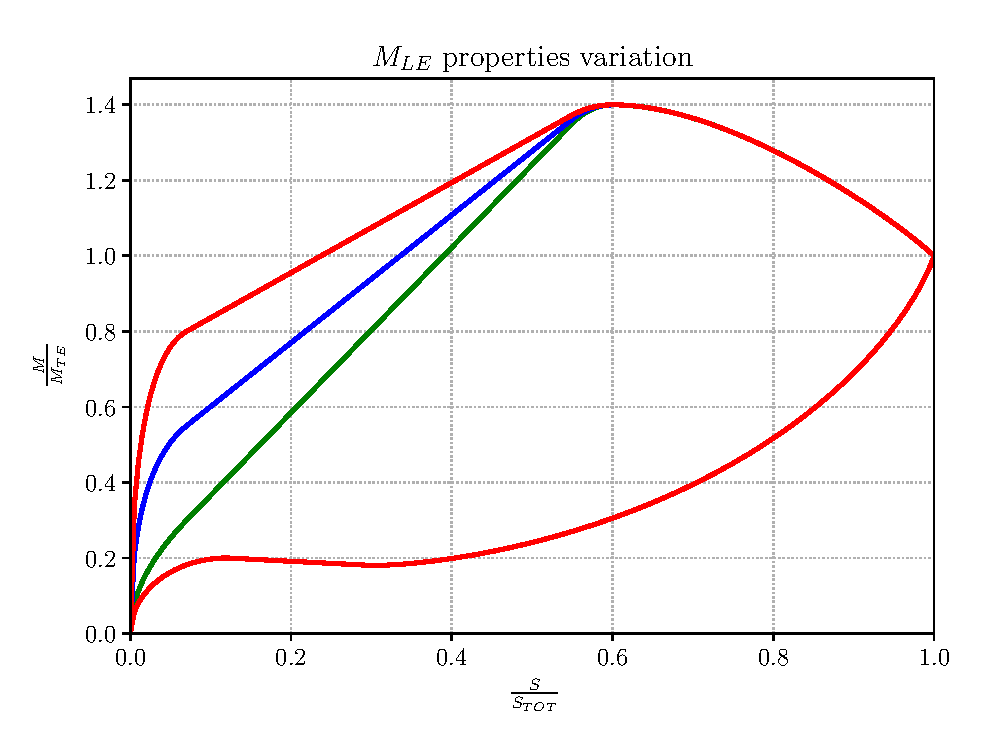
\includegraphics[width=\width\textwidth]{pyFigure/figures/load-MLE.eps}
    \caption{$\frac{M}{M_{TE}} \ vs \ \frac{S}{S_{TOT}}$. $M_{LE}$ variation.}    
    \label{fig:MLE}
\end{figure}

\begin{figure}[!h]
    \centering
    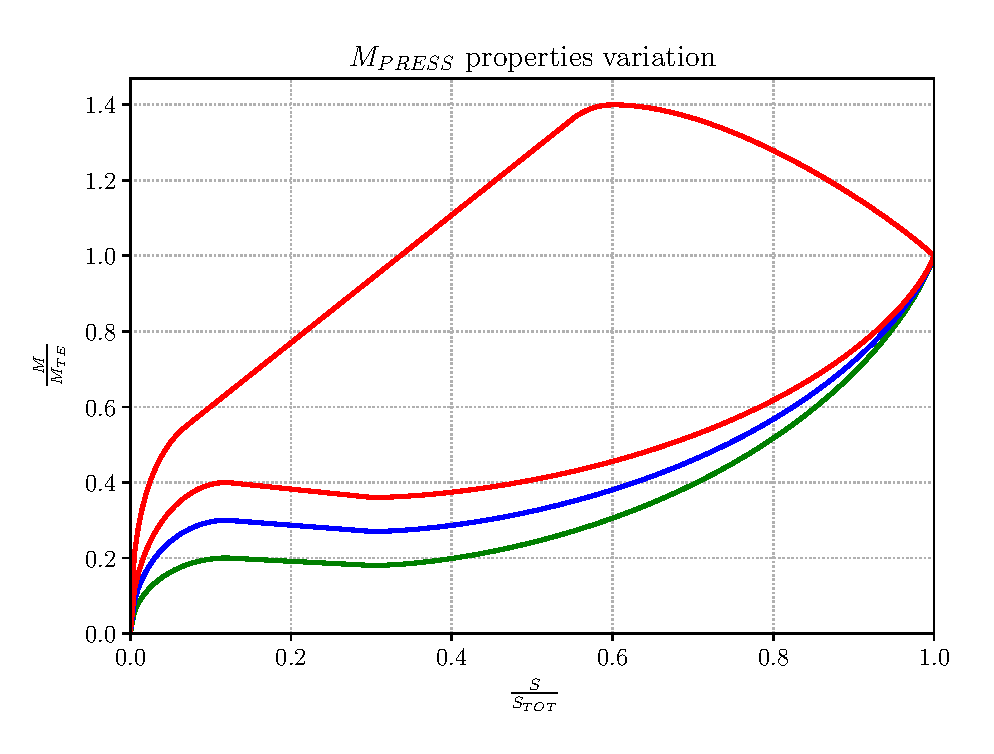
\includegraphics[width=\width\textwidth]{pyFigure/figures/load-MPRESS.eps}
    \caption{$\frac{M}{M_{TE}} \ vs \ \frac{S}{S_{TOT}}$. $M_{PRESS}$ variation.}    
    \label{fig:MPRESS}
\end{figure}

\begin{figure}[!h]
    \centering
    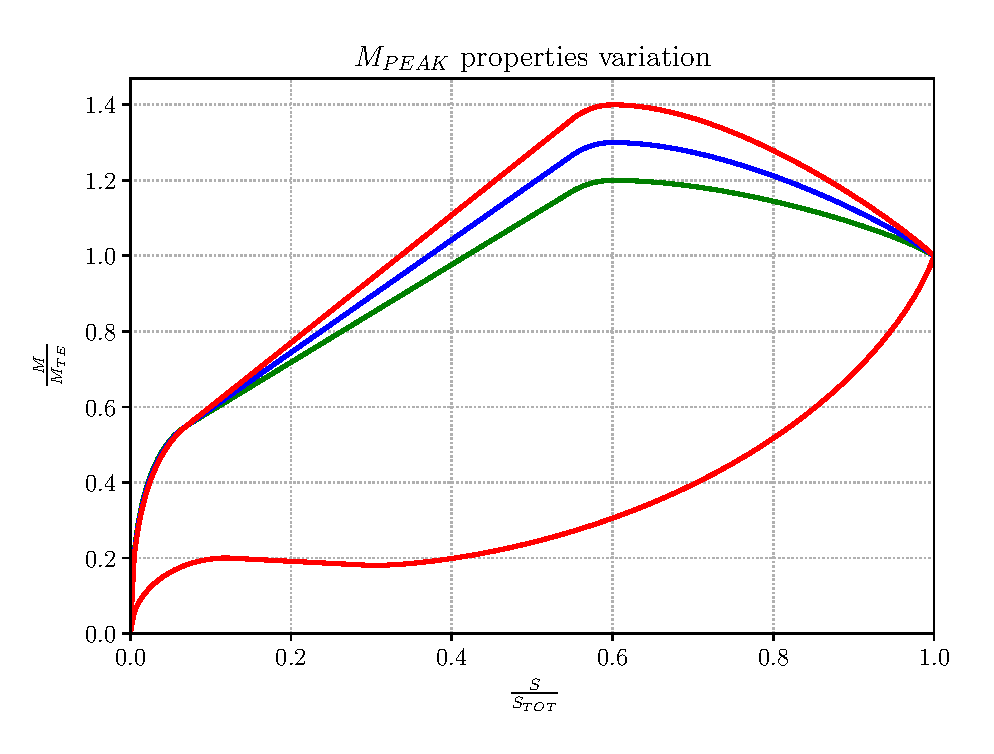
\includegraphics[width=\width\textwidth]{pyFigure/figures/load-MPEAK.eps}
    \caption{$\frac{M}{M_{TE}} \ vs \ \frac{S}{S_{TOT}}$. $M_{PEAK}$ variation.}    
    \label{fig:MPEAK}
\end{figure}

\begin{figure}[!h]
    \centering
    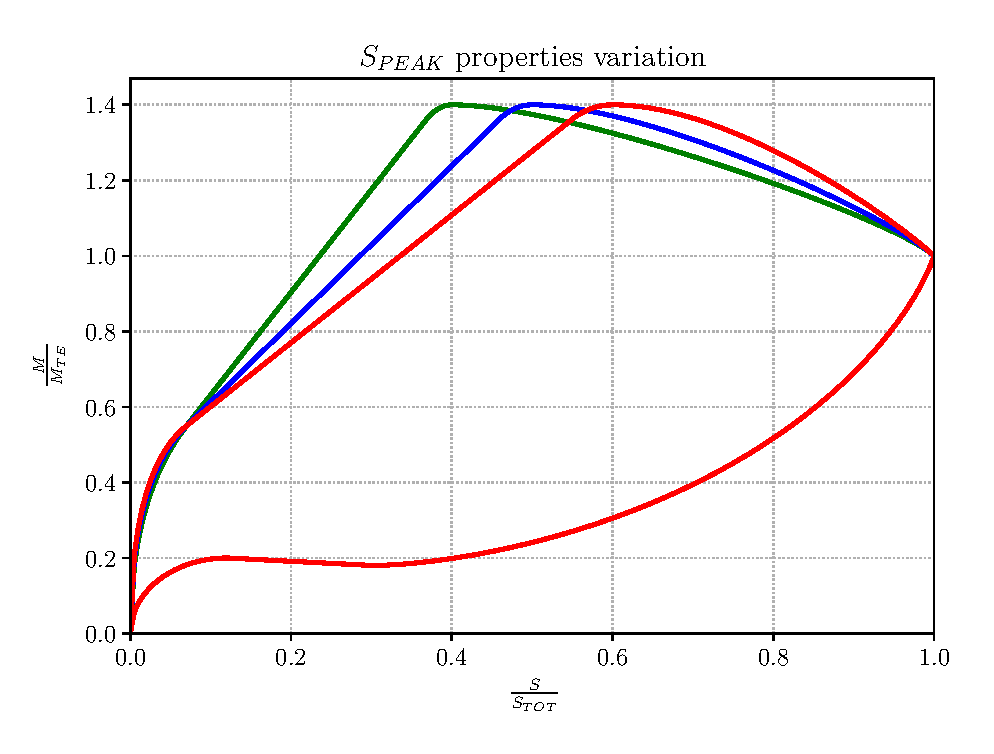
\includegraphics[width=\width\textwidth]{pyFigure/figures/load-SPEAK.eps}
    \caption{$\frac{M}{M_{TE}} \ vs \ \frac{S}{S_{TOT}}$. $S_{PEAK}$ variation.}    
    \label{fig:SPEAK}
\end{figure}

\subsubsection{Blade Geometry}

The blade geometry - consisting of the camberline, suction side and pressure side - is defined through meticulous parametrization, following Kulfan's approach. 

\begin{figure}[!h]
    \centering 
    \hspace*{-1.7cm}
    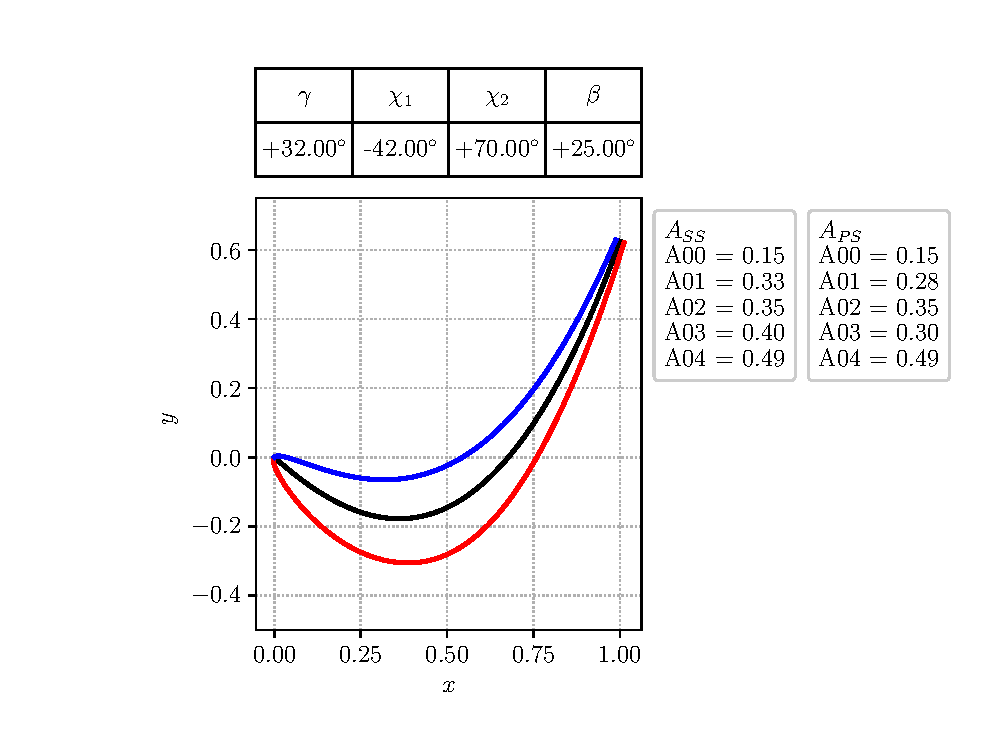
\includegraphics[width=0.6\textwidth]{pyFigure/figures/blade.eps}
    \caption{Kulfan parametrized blade.}
    \label{fig:blade}
\end{figure}

\begin{figure}[!h]
    \centering 
    \hspace*{-1.7cm}
    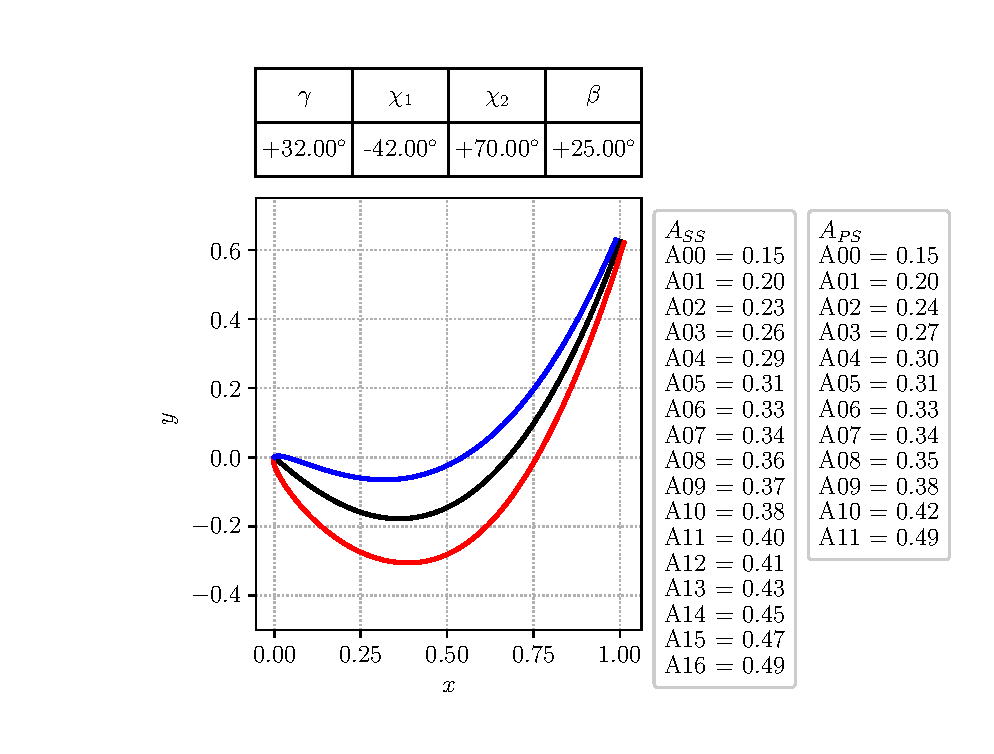
\includegraphics[width=0.6\textwidth]{pyFigure/figures/scaledBlade.eps}
    \caption{Figure~\ref{fig:blade} scaled blade with a higher parametrization.}
    \label{fig:scaledBlade}
\end{figure}

% The camberline is parametrized by the stagger angle ($\gamma$), the metal inlet angle ($\chi_1$), and the metal outlet angle ($\chi_2$). 
% The suction side and the pressure side of the blade are defined using a set of $N$ parameters, $A_i$.
% A blade can be scaled using more parameters by simply solving a linear system of equations. 
% Kulfan's parametrization retains critical geometric properties, including leading edge radius ($R_{LE}$) and trailing edge angle ($\beta$), significantly influencing blade characteristics and flow properties. 

The camberline is parameterized by the stagger angle ($\gamma$), the metal inlet angle ($\chi_1$), and the metal outlet angle ($\chi_2$). The suction side and the pressure side of the blade are defined using a set of $N$ parameters, $A_i$. Scaling a blade can be accomplished using additional parameters by solving a linear system of equations.

Kulfan's parametrization~\cite{kulfan2008universal} preserves critical geometric properties, including the leading-edge radius ($R_{LE}$) and the trailing-edge angle ($\beta$), which have a significant impact on blade characteristics and flow properties.

Figure~\ref{fig:blade} and Figure~\ref{fig:scaledBlade} show the Kulfan parametrized blade and the same blade scaled with a higher parametrization.

\subsection{Database Generation}

% The database is made using an in-house made code designed for the blade optimization and analysis, aptly named \texttt{datablade}. The program structure is modular, allowing for versatile combinations of blocks tailored to specific objectives.
The database is created using an in-house code designed for blade optimization and analysis, appropriately named \texttt{datablade}. The program's structure is modular, enabling flexible combinations of blocks tailored to specific objectives.

\subsubsection{Configuration File}

% \texttt{datablade} optimization relies on a configuration file, formatted in \texttt{.json} for enhanced readability and ease of use. This file serves as the blueprint for blade optimization, initializing parameters such as the initial guess for blade geometry, geometrical constraints setup and loading properties. 
\texttt{datablade} optimization relies on a configuration file, formatted in \texttt{.json} for enhanced readability and ease of use. This file serves as the blueprint for blade optimization, initializing parameters such as the initial guess for blade geometry, geometrical constraints setup, and loading properties.

\subsubsection{Optimization}

% The blade optimization plays a pivotal role, employing a classic gradient-free method known as the Simplex method. This method, while finding local minima, yields satisfactory results when guided by appropriate initial guesses, dimensionality adaptation strategies, and a robust cost function.
The blade optimization plays a pivotal role, employing a classic gradient-free method known as the Simplex method. This method, while seeking local minima, delivers satisfactory results when guided by suitable initial guesses, dimensionality adaptation strategies, and a robust cost function.

\paragraph{Dimensionality Adaptation}

% Optimizing blades involves solving multidimensional optimization problems with complex solutions. \texttt{datablade} adopts an intelligent strategy that adjusts the problem's dimensionality. Initially, optimization begins with fewer parameters to flatten the design space. Upon achieving convergence, the degree of freedom is increased incrementally, leading to improved solutions. Empirical tests have validated this approach, showcasing its effectiveness in constructing the database.
Optimizing blades involves solving multidimensional optimization problems with complex solutions. \texttt{datablade} adopts an intelligent strategy that adjusts the problem's dimensionality. Initially, optimization commences with fewer parameters to reduce the design space. As convergence is achieved, the degree of freedom is incrementally increased, leading to improved solutions. Empirical tests have validated this approach, demonstrating its effectiveness in constructing the database.

\paragraph{Cost Function}

% The heart of blade optimization lies in managing two primary errors: load distribution and flow exit angle. These errors are quantified using the root mean squared error ($RMSE$) and the flow exit angle error ($\Delta \alpha_2$). The cost function, a blend of these properties, establishes guidelines for optimization convergence and acceptance thresholds for optimized blades. The function balances the importance of angle error ($\Delta \alpha_2$) relative to $RMSE$ using scaling and threshold values.
The core of blade optimization revolves around the management of two key errors: load distribution and flow exit angle. These errors are quantified using the root mean squared error ($RMSE$) and the flow exit angle error ($\Delta \alpha_2$). The cost function, which combines these properties, sets criteria for optimization convergence and establishes acceptance thresholds for optimized blades. The function balances the significance of the angle error ($\Delta \alpha_2$) relative to $RMSE$ through the use of scaling and threshold values.

{\scriptsize
\begin{align}
    & RMSE             = \sqrt{\frac{1}{N} \cdot \sum_{i = 1}^{N} \Bigg( \frac{M_{real}}{M_{TE, real}} \Bigg|_{i} - \frac{M_{target}}{M_{TE, target}} \Bigg|_{i} \Bigg)^2} 
    \label{eqn:RMSE}
    \\ 
    & \Delta \alpha_2  = \Big| \alpha_{2, real} - \alpha_{2, target} \Big| 
    \label{eqn:angleError}
    \\
    & cost             = RMSE \cdot \Big[ 1 + 0.04 \cdot \Big( max \Big( 0, \ \Delta \alpha_2 - 1.0 \Big) \Big)^{2.0} \Big]
    \label{eqn:costFunction}
\end{align}
}

\subsubsection{Optimizer}

% The \texttt{datablade} optimizer combines the capabilities of the \texttt{MISES} software - for the flow properties computation - with the \texttt{scipy} module, offering robust performance and efficiency. 
The \texttt{datablade} optimizer combines the capabilities of the \texttt{MISES} software~\cite{drela1998user} for flow properties computation with the \texttt{scipy} module using the Simplex method~\cite{nelder1965simplex}, providing robust performance and efficiency.

\subsubsection{Domain}

\begin{table}[!h]
    \caption{Domain boundaries and discretization.}
    \label{tab:domain}
    \begin{center}
        \renewcommand{\arraystretch}{2}
        \begin{tabularx}{0.45\textwidth} { 
            | >{\centering\arraybackslash}X 
            | >{\centering\arraybackslash}X 
            | >{\centering\arraybackslash}X 
            | >{\centering\arraybackslash}X | } 
            \hline
            % \rowcolor{bluepoli!40}
            \textbf{Variable} & \textbf{Min} & \textbf{Max} & \textbf{Points} \\ [0.5ex] 
            \hline\hline
            $\alpha_1$ & $-50^{\circ}$ & $-20^{\circ}$ & 3 \\ [0.5ex]
            \hline
            $\alpha_2$ & $65^{\circ}$ & $72.5^{\circ}$ & 4 \\ [0.5ex]
            \hline
            $M_2$ & $0.4$ & $0.7$ & 3 \\ [0.5ex]
            \hline
            $Re$ & $6 \cdot 10^5$ & $6 \cdot 10^5$ & 1 \\ [0.5ex] 
            \hline
            $\frac{M_P}{M_{TE}}$ & $1.2$ & $1.4$ & 3 \\ [0.5ex]
            \hline
            $\frac{L_P}{L_{surf}}$ & $0.5$ & $0.6$ & 3 \\ [0.5ex]
            \hline
            $\frac{M_{LE}}{M_{TE}}\frac{M_2}{M_1}$ & $1.2$ & $1.8$ & 3 \\ [0.5ex]
            \hline
            $\frac{M_{PS}}{M_{TE}}\frac{M_2}{M_{1, ax}}$ & $0.8$ & $1.2$ & 3 \\ 
            \hline
        \end{tabularx}
    \end{center}
\end{table}

% The database is made by optimizing blades with different aerodynamic style and aerodynamic duty properties. 
% The dataset points are shown in Table~\ref{tab:domain}.
% Due the study of the high pressure turbine, a fixed Reynolds number ($Re = 6 \cdot 10^5$) is employed due to the Reynolds independence of the flow under investigation.
% A novel optimization strategy unfolds as an additional acceleration layer for computing the initial guess ($\boldsymbol{x}_0$) used in the optimizer. This strategy involves linearizing the inner domain using data from outer domain points. The outer points are optimized first to provide a suitable initial guess for inner domain points, streamlining the overall convergence speed of the database.
The database is created by optimizing blades with different aerodynamic styles and aerodynamic duty properties. 
The dataset points are presented in Table~\ref{tab:domain}.

For the high-pressure turbine study, a fixed Reynolds number ($Re = 6 \times 10^5$) is employed due to the Reynolds independence of the flow under investigation.

An innovative optimization strategy unfolds as an additional acceleration layer for computing the initial guess ($\boldsymbol{x}_0$) used in the optimizer. This strategy involves linearizing the inner domain using data from outer domain points. The outer points are optimized first to provide a suitable initial guess for inner domain points, thereby streamlining the overall convergence speed of the database~\cite{clark2019step}.

\paragraph{Outer Points}

% Generating the corner points of the domain is the initial and time-consuming step in database creation. These corner points serve as a foundation, accelerating the optimization process for inner domain points. \texttt{datablade} optimizes 128 blades to establish these corner points.
% Figure~\ref{fig:linearInterpolation} represents the boundary points of the domain of study.

Generating the corner points of the domain is the initial and time-consuming step in database creation. These corner points serve as a foundation, expediting the optimization process for inner domain points. \texttt{datablade} optimizes 128 blades to establish these corner points.

Figure~\ref{fig:linearInterpolation} illustrates the boundary points of the study domain.

\begin{figure}[!h]
    \centering
    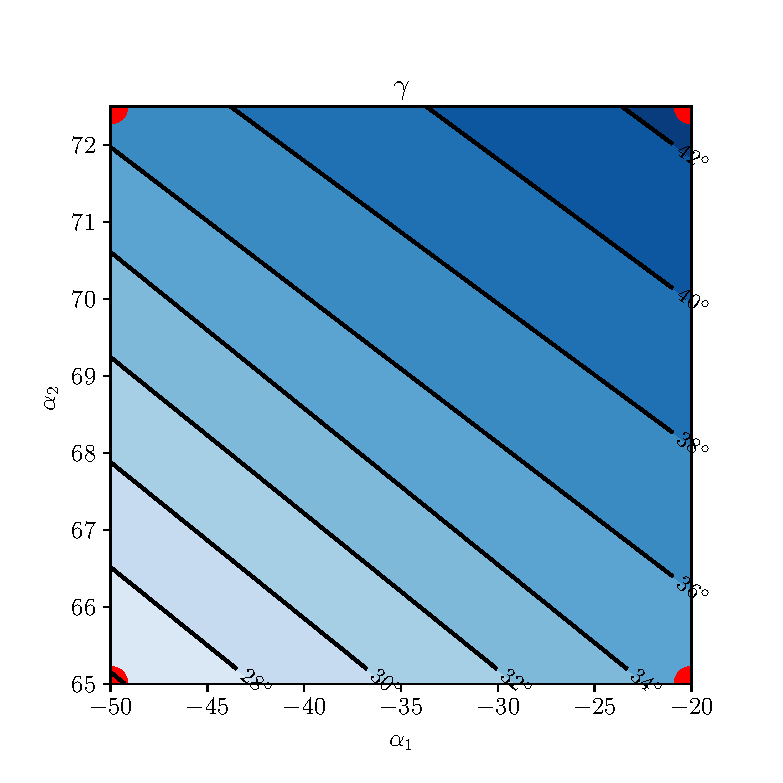
\includegraphics[width=0.5\textwidth]{./images/staggerLinear.eps}
    \caption{Linear interpolation of the stagger angle, $\gamma$, with respect to $\alpha_1$ and $\alpha_2$ from the corner points in red.}
    \label{fig:linearInterpolation}
\end{figure}

\paragraph{Inner Points}

% Following the creation of corner points, inner points initial guess, $\boldsymbol{x}_0$, are computed using linear interpolation. This approach facilitates the estimation of blade parameters for the entire inner domain. The chapter outlines the linear interpolation process applied to all blade parameters. A total of 2916 blades will be optimized for inner points, completing the comprehensive database.
% Figure~\ref{fig:linearInterpolationFinal} shows the initial guess, $\gamma$, from a linear interpolation of the domain.

After generating the corner points, the initial guess for inner points, denoted as $\boldsymbol{x}_0$, is computed using linear interpolation. This method simplifies the estimation of blade parameters across the entire inner domain. A total of 2916 blades will undergo optimization for inner points, culminating in the creation of the comprehensive database.

Figure~\ref{fig:linearInterpolationFinal} displays the initial guess, $\gamma$, obtained through linear interpolation of the domain.

\begin{figure}[!h]
    \centering
    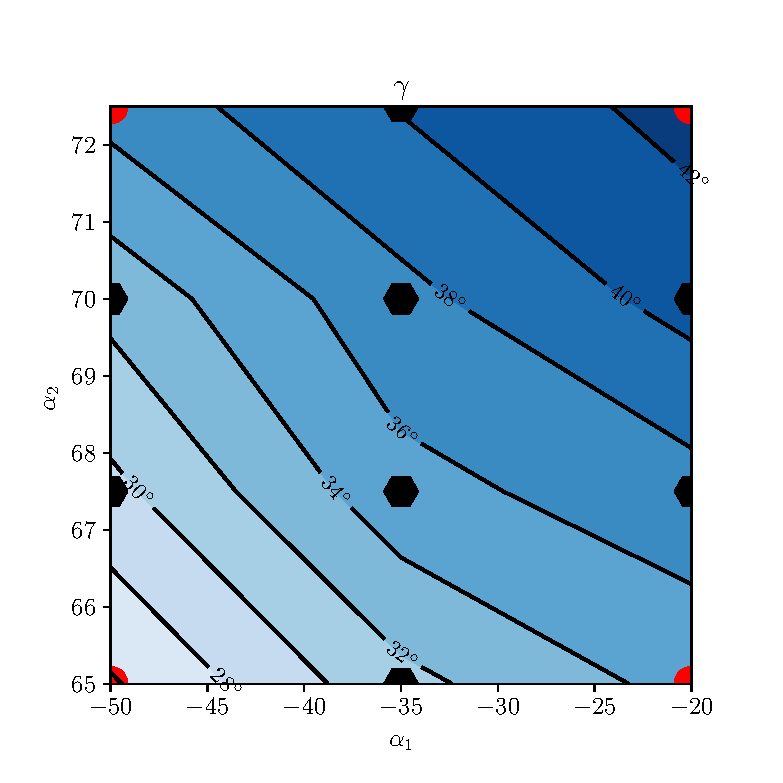
\includegraphics[width=0.5\textwidth]{./images/staggerComplete.eps}
    \caption{Complete $\gamma$ variation with respect to $\alpha_1$ \& $\alpha_2$. Corner points in red and inner points in black.}
    \label{fig:linearInterpolationFinal}
\end{figure}

\subsubsection{Optimized Data}

\begin{table}[!h]  
    \centering
    \renewcommand{\arraystretch}{2}
    \caption{Data properties inside the optimized database.}
    \label{tab:database}
    \begin{tabularx}{0.45\textwidth} { 
        | >{\centering\arraybackslash}X 
         >{\centering\arraybackslash}X 
         >{\centering\arraybackslash}X
         >{\centering\arraybackslash}X
         >{\centering\arraybackslash}X
         >{\centering\arraybackslash}X | } 
        \hline
                                       & $\boldsymbol{count}$ & $\boldsymbol{\mu}$ & $\boldsymbol{\sigma}$ & $\boldsymbol{min}$  & $\boldsymbol{max}$ \\ \hline\hline
        $\boldsymbol{cost}$            & $2916$               & $0.01$             & $0.006$               & $0.005$             & $0.04$             \\ \hline
        $\boldsymbol{\Delta \alpha_2}$ & $2916$               & $0.96^\circ$       & $0.542^\circ$         & $0.0003^\circ$       & $2.37^\circ$       \\ \hline
    \end{tabularx}
\end{table}

% The database holds Kulfan's parameters defining blade geometry. Key blades of interest for initial analysis are categorized based on their loading distribution and exit flow angle errors:

% \begin{itemize}
%     \item Blades with low error on the loading distribution and low error on the exit flow angle. Figure~\ref{fig:goodBlade} shows this blade setup.
%     \item Blades with low error on the loading distribution but high error on the exit flow angle. Figure~\ref{fig:midBlade} shows this blade behavior.
%     \item Blades with high error on both the loading distribution and the exit flow angle. Figure~\ref{fig:badBlade} shows this blade family.
% \end{itemize}

The database contains Kulfan's parameters that define blade geometry. Key blades of interest for initial analysis are categorized based on their loading distribution and exit flow angle errors:

\begin{itemize}
    \item Blades with low errors in both the loading distribution and the exit flow angle. Figure~\ref{fig:goodBlade} illustrates this blade setup.
    \item Blades with low errors in the loading distribution but high errors in the exit flow angle. Figure~\ref{fig:midBlade} represents this blade behavior.
    \item Blades with high errors in both the loading distribution and the exit flow angle. Figure~\ref{fig:badBlade} depicts this blade family.
\end{itemize}

\begin{figure}[!h]
    \centering
    \hspace*{-0.6cm}
    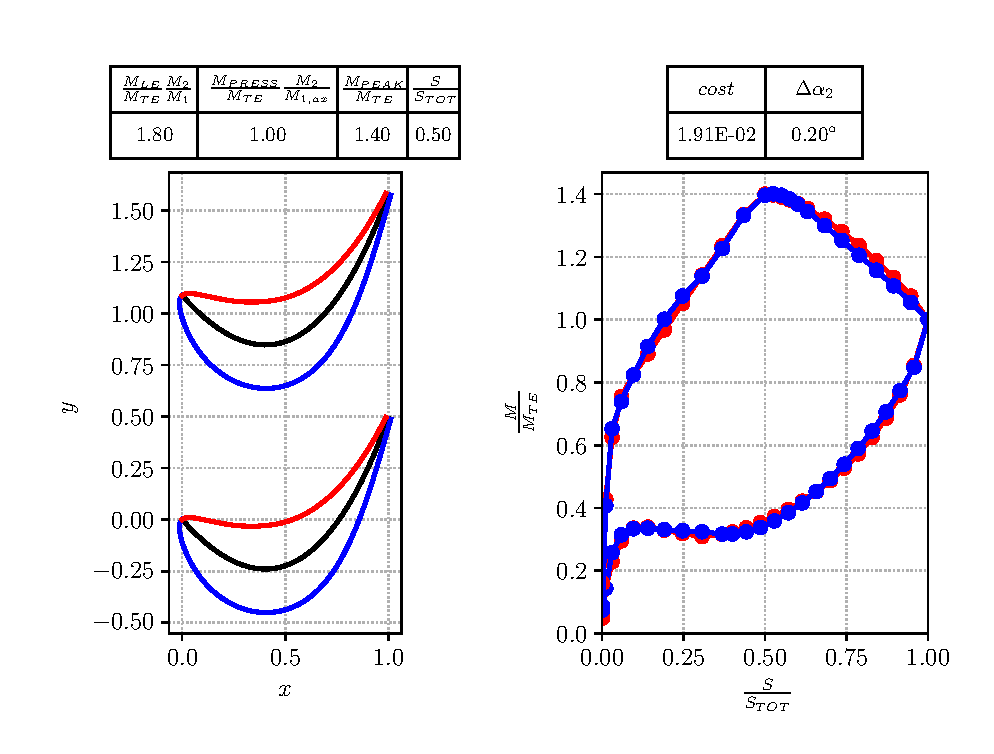
\includegraphics[width=0.45\textwidth]{./images/bladeVal0305.eps}
    \caption{Blade with good performances on the load distribution and on the exit angle error.}
    \label{fig:goodBlade}
\end{figure}

\begin{figure}[!h]
    \centering 
    \hspace*{-0.6cm}
    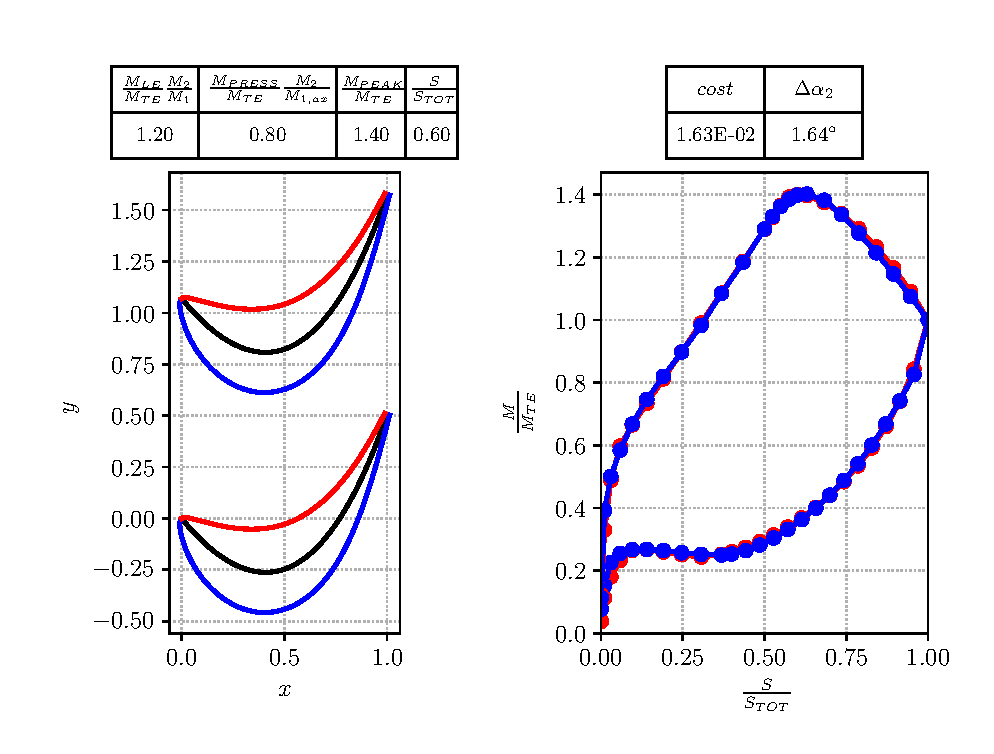
\includegraphics[width=0.45\textwidth]{./images/bladeVal0477.eps}
    \caption{Blade with good performances on the load distribution but low performance on the exit angle error.}
    \label{fig:midBlade}
\end{figure}

\begin{figure}[!h]
    \centering
    \hspace*{-0.6cm}
    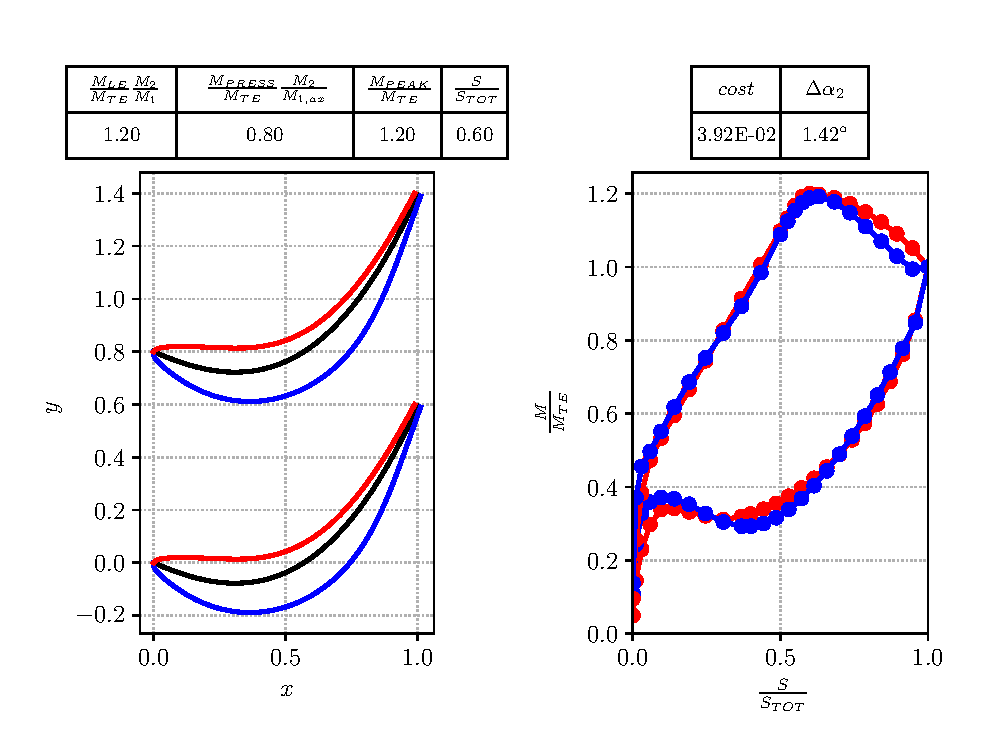
\includegraphics[width=0.45\textwidth]{./images/bladeVal1962.eps}
    \caption{Blade with poor performances on the load distribution and on the exit angle error.}
    \label{fig:badBlade}
\end{figure}

% Table~\ref{tab:database} provides an overview of the complete database after optimization, demonstrating acceptable mean values for cost and $\Delta \alpha_2$. A significant portion of the blades exhibit a cost below $2.75\%$, suggesting convergence toward the desired aerodynamic style. However, it's noted that more than $25\%$ of the database has an exit flow angle error, $\Delta \alpha_2$, exceeding $1^{\circ}$, highlighting the need for correction.
% Some blades perform poorly, these are excluded from the machine learning analysis due to high discrepancies in loading distribution. These blades lack correlation with the desired aerodynamic style.

Table~\ref{tab:database} provides an overview of the complete database after optimization, showcasing acceptable mean values for cost and $\Delta \alpha_2$. A significant portion of the blades demonstrates a cost below $2.75\%$, indicating convergence towards the desired aerodynamic style. However, it is worth noting that over $25\%$ of the database exhibits an exit flow angle error, $\Delta \alpha_2$, exceeding $1^{\circ}$, underscoring the need for correction.

Some blades perform poorly and are excluded from the machine learning analysis due to significant discrepancies in loading distribution. These blades lack correlation with the desired aerodynamic style.

\subsubsection{Error Distribution}

% Certain blades within the database present significant errors in the loading distribution ($RMSE$). These unfeasible designs, marked by bad input data, cannot be rectified by machine learning algorithms. Consequently, unfeasible designs are omitted from the database to provide meaningful data for interpolation.
% Figure~\ref{fig:errorDistribution1} and Figure~\ref{fig:angleError} show the error distribution on a \textit{slice} of the domain.

Certain blades within the database exhibit significant errors in the loading distribution ($RMSE$). These infeasible designs, characterized by erroneous input data, cannot be rectified by machine learning algorithms. As a result, infeasible designs are excluded from the database to ensure the availability of meaningful data for interpolation. A threshold of $2.75\%$ is used as filter for refining the database.

Figure~\ref{fig:errorDistribution1} and Figure~\ref{fig:angleError} illustrate the error distribution on a \textit{slice} of the domain.

\begin{figure}[!h]
    \centering
    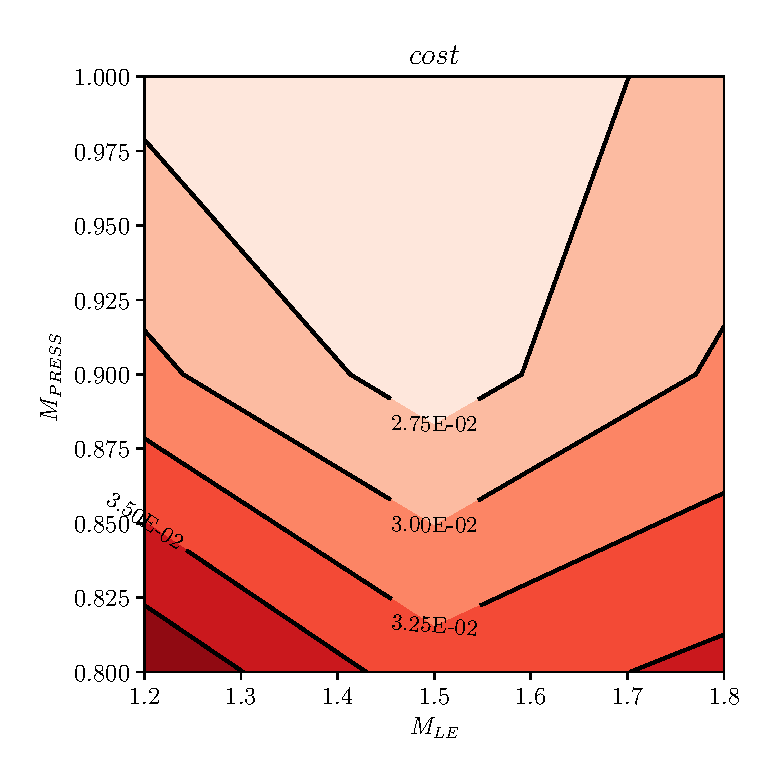
\includegraphics[width=0.5\textwidth]{./images/costError1.eps}
    \caption{$cost$ distribution.}
    \label{fig:errorDistribution1}
\end{figure}

\begin{figure}[!h]
    \centering
    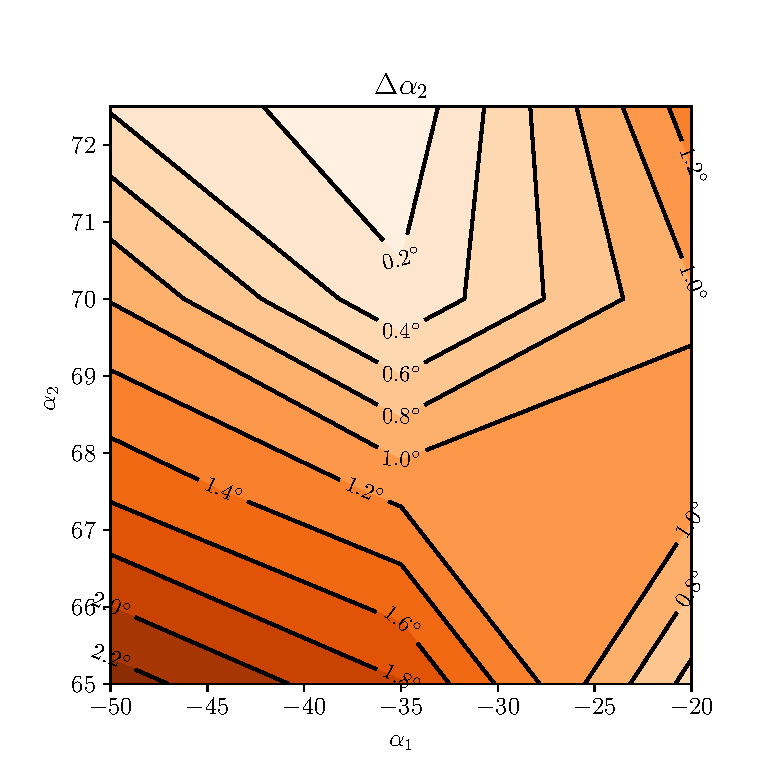
\includegraphics[width=0.5\textwidth]{./images/angleError.eps}
    \caption{$\Delta \alpha_2$ behavior in the domain.}
    \label{fig:angleError}
\end{figure}

\subsubsection{Filtering}

% To refine the database for interpolation purposes, data filtering is employed. Blades with inadmissible errors in blade loading are excluded, reducing the dataset slightly. The unfeasible designs are primarily situated at the boundaries of the domain, warranting their exclusion. The filtering process is primarily based on the cost properties of the blade, as it predominantly reflects $RMSE$.
% Blades with low $RMSE$ but high $\Delta \alpha_2$ will then be filtered numerically by the machine learning algorithm with a correction of the blade design function, $\hat{\mathnormal{f}}$.
% Table~\ref{tab:filteredDatabase} shows the database properties after the filtering operation.
To refine the database for interpolation purposes, data filtering is implemented. Blades with unacceptable errors in blade loading are omitted, resulting in a slight reduction in the dataset. The infeasible designs are typically located at the domain boundaries, justifying their exclusion. The filtering process primarily relies on the blade's cost properties, as it predominantly reflects the $RMSE$.

Blades with low $RMSE$ but high $\Delta \alpha_2$ will be subsequently filtered numerically by the machine learning algorithm through a correction of the blade design function, $\hat{\mathnormal{f}}$.

Table~\ref{tab:filteredDatabase} displays the database properties following the filtering operation.

\begin{table}[!h]  
    \centering
    \renewcommand{\arraystretch}{2}
    \caption{Data properties inside the optimized database.}
    \label{tab:filteredDatabase}
    \begin{tabularx}{0.45\textwidth} { 
        | >{\centering\arraybackslash}X 
         >{\centering\arraybackslash}X 
         >{\centering\arraybackslash}X
         >{\centering\arraybackslash}X
         >{\centering\arraybackslash}X
         >{\centering\arraybackslash}X | } 
        \hline
                                       & $\boldsymbol{count}$ & $\boldsymbol{\mu}$ & $\boldsymbol{\sigma}$ & $\boldsymbol{min}$ & $\boldsymbol{max}$ \\ \hline\hline
        $\boldsymbol{cost}$            & $2787$               & $0.015$         & $0.004$            & $0.005$         & $0.027$         \\ \hline
        $\boldsymbol{\Delta \alpha_2}$ & $2787$               & $0.846^\circ$   & $0.421^\circ$      & $0.001^\circ$   & $2.373^\circ$   \\ \hline
    \end{tabularx}
\end{table}

\section{Machine Learning}

% The core of the machine learning algorithm is built upon regression techniques, specifically tailored for domain interpolation. This algorithm performs the remarkable task of predicting blade geometries based on inputs of aerodynamic duty and aerodynamic style, mirroring the parameterization of the database's blades.

% The domains of study:
% \begin{itemize}
%     \item $\mathcal{X}$: this dataset stores the aerodynamic style and aerodynamic duty properties, organized as $\mathcal{X} \in \mathbb{R}^{2787 \times 8}$, signifying $2787$ filtered blades and $8$ parameters responsible for delineating the aerodynamic style and duty. The $\boldsymbol{x}$ vector stores the aerodyanmic style and aerodynamic duty of the blade and it is the general element within $\mathcal{X}$.
%     \item $\mathcal{Y}$: this dataset stores the camberline and Kulfan parameters, essential for characterizing each blade. It is structured as $\mathcal{Y} \in \mathbb{R}^{2787 \times 42}$, denoting $2787$ blades and $42$ parameters, including Kulfan parameters and pitch. The $\boldsymbol{y}$ vector stores the blade geometry properties and it is the general element within $\mathcal{Y}$.
% \end{itemize}
% The machine learning algorithm is entrusted with the task of approximating a mapping function, $\mathnormal{f}$, which bridges the two domains, $\mathcal{X}$ and $\mathcal{Y}$, as illustrated in Equation~\ref{eqn:mapFuncML}.

% The subsequent endeavor revolves around computing $\hat{\mathnormal{f}}$, a numerical approximation of $\mathnormal{f}$. This new function, $\hat{\mathnormal{f}}$ plays a pivotal role in defining the underlying problem.

The heart of the machine learning algorithm is constructed upon regression techniques, specifically tailored for domain interpolation. This algorithm excels in the remarkable task of predicting blade geometries based on inputs of aerodynamic duty and aerodynamic style, mirroring the parameterization of the database's blades.

The domains of study are as follows:
\begin{itemize}
    \item $\mathcal{X}$: This dataset stores the aerodynamic style and aerodynamic duty properties, organized as $\mathcal{X} \in \mathbb{R}^{2787 \times 8}$, representing $2787$ filtered blades and $8$ parameters responsible for defining the aerodynamic style and duty. The $\boldsymbol{x}$ vector holds the aerodynamic style and aerodynamic duty of the blade and is a general element within $\mathcal{X}$.
    \item $\mathcal{Y}$: This dataset stores the camberline and Kulfan parameters, essential for characterizing each blade. It is structured as $\mathcal{Y} \in \mathbb{R}^{2787 \times 42}$, indicating $2787$ blades and $42$ parameters, including Kulfan parameters and pitch. The $\boldsymbol{y}$ vector encompasses the blade geometry properties and is a general element within $\mathcal{Y}$.
\end{itemize}

The machine learning algorithm is tasked with approximating a mapping function, $\mathnormal{f}$, which bridges the two domains, $\mathcal{X}$ and $\mathcal{Y}$, as depicted in Equation~\ref{eqn:mapFunc}.

The subsequent endeavor revolves around computing $\hat{\mathnormal{f}}$, a numerical approximation of $\mathnormal{f}$. This new function, $\hat{\mathnormal{f}}$, plays a pivotal role in defining the underlying problem.

\begin{align}
    \mathnormal{f}_{(\boldsymbol{x})} = \boldsymbol{y}
    \label{eqn:mapFunc} \\
    \hat{\mathnormal{f}}_{(\boldsymbol{x})} \approx \boldsymbol{y}
    \label{eqn:mapFuncML}
\end{align}

\subsection{Radial Basis Function}

% To achieve the goals, the choice of a suitable regression algorithm is imperative. In this research, radial basis functions (RBFs) are selected as the kernel of the machine learning model. RBFs, renowned for their robustness, prove to be a powerful tool for data interpolation. They adeptly manage overfitting issues and facilitate perfect interpolation of training points $(\boldsymbol{x}^*, \boldsymbol{y}^*)$. The kernel relies on parameters like length scale and the Euclidean norm between domain points, which contribute to its effectiveness in minimizing the influence of distant data points.
% The application of Gaussian functions in approximating the domain is another significant aspect, ensuring the smooth transition of geometrical properties of the blade, including camberline and Kulfan parameters. 
To achieve the research goals, the selection of a suitable regression algorithm is crucial. In this study, radial basis functions (RBFs) are chosen as the kernel for the machine learning model. RBFs, known for their robustness, prove to be a powerful tool for data interpolation~\cite{geron2022hands}. They effectively handle overfitting issues and enable perfect interpolation of training points $(\boldsymbol{x}^*, \boldsymbol{y}^*)$. The kernel relies on parameters such as length scale and the Euclidean norm between domain points, which contribute to its effectiveness in minimizing the influence of distant data points.

The utilization of Gaussian functions to approximate the domain is another significant aspect, ensuring the smooth transition of geometrical properties of the blade, including camberline and Kulfan parameters.

\subsection{Training \& Testing}

% With the fundamentals in place, the work proceeds to construct a system for the computation of $\hat{\mathnormal{f}}$. This system is characterized by a linear system of equations, representing linear combinations of radial basis functions. These equations are weighted by parameters referred to as weights, $\boldsymbol{w}$, which are integral to fitting the radial basis functions into the database.

% Once $\boldsymbol{w}$ is computed, the chapter delves into the evaluation of weight quality using the test set $(\mathcal{X}^{**}, \mathcal{Y}^{**})$.

% Figure~\ref{fig:bladeML1}, Figure~\ref{fig:bladeML3} and Figure~\ref{fig:bladeML4} showblades generated from $\hat{\mathnormal{f}}$. It can be seen that the error over the $RMSE$ stays always lower than $3 \cdot 10^{-2}$ and the $\Delta \alpha_2$ is always lower than $0.5^{\circ}$.
% These results are acceptable for the purpose of the design tool generated by this work.
With the foundational elements in place, the work progresses to establish a system for computing $\hat{\mathnormal{f}}$. This system is characterized by a linear system of equations, representing linear combinations of radial basis functions. These equations are weighted by parameters referred to as weights, denoted as $\boldsymbol{w}$, which are essential for fitting the radial basis functions to the database.

Once $\boldsymbol{w}$ is computed, the chapter delves into evaluating the quality of weights using the test set $(\mathcal{X}^{**}, \mathcal{Y}^{**})$.

Figure~\ref{fig:bladeML1}, Figure~\ref{fig:bladeML3}, and Figure~\ref{fig:bladeML4} display blades generated from $\hat{\mathnormal{f}}$. It can be observed that the error in $RMSE$ consistently remains below $3 \cdot 10^{-2}$, and $\Delta \alpha_2$ is consistently lower than $0.5^{\circ}$. These results are deemed acceptable for the purpose of the design tool generated by this work.

\begin{figure}[!h]
    \centering 
    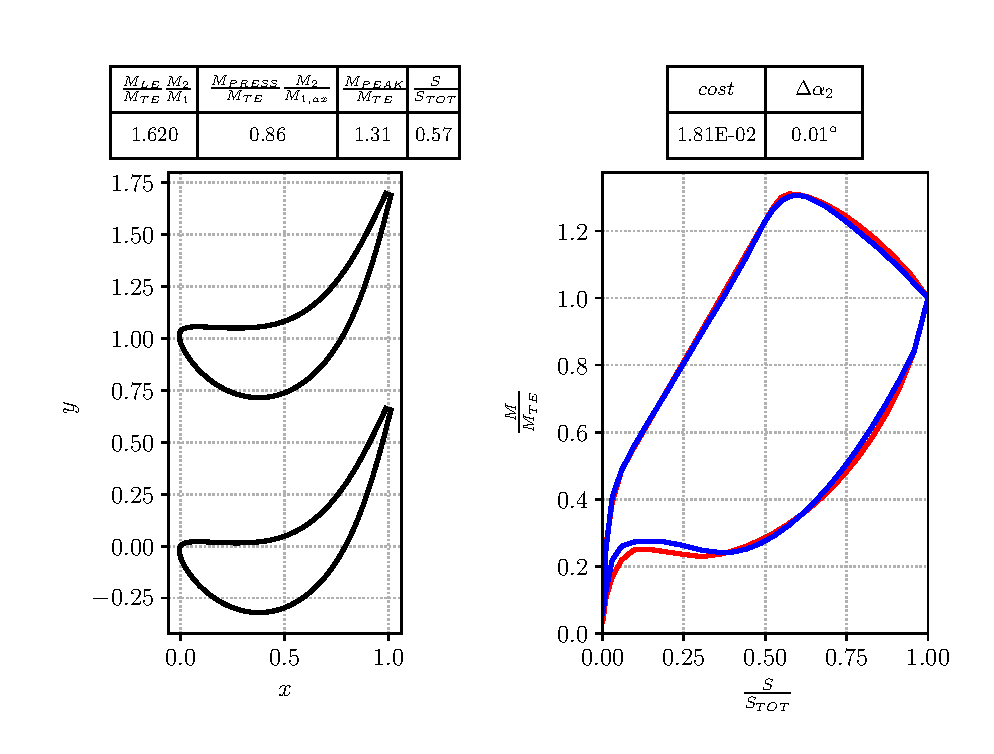
\includegraphics[width=\widthPCA\textwidth]{./images/blade--3404-7015-57.eps}
    \caption{Blade generated by $\hat{\mathnormal{f}}$ with $\alpha_1 = -34.04^{\circ}$, $\alpha_2 = 70.15^{\circ}$ and $M_2 = 0.57$.}
    \label{fig:bladeML1}
\end{figure}

\begin{figure}[!h]
    \centering 
    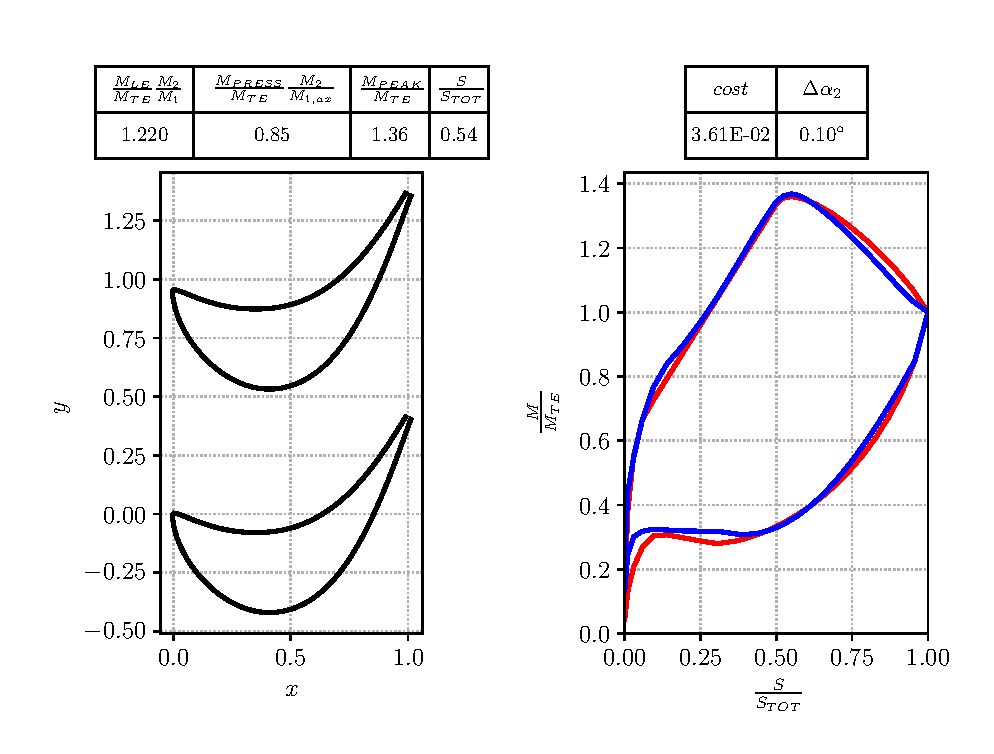
\includegraphics[width=\widthPCA\textwidth]{./images/blade--4916-6516-67.eps}
    \caption{Blade generated by $\hat{\mathnormal{f}}$ with $\alpha_1 = -49.16^{\circ}$, $\alpha_2 = 65.16^{\circ}$ and $M_2 = 0.67$.}
    \label{fig:bladeML3}
\end{figure}

\begin{figure}[!h]
    \centering 
    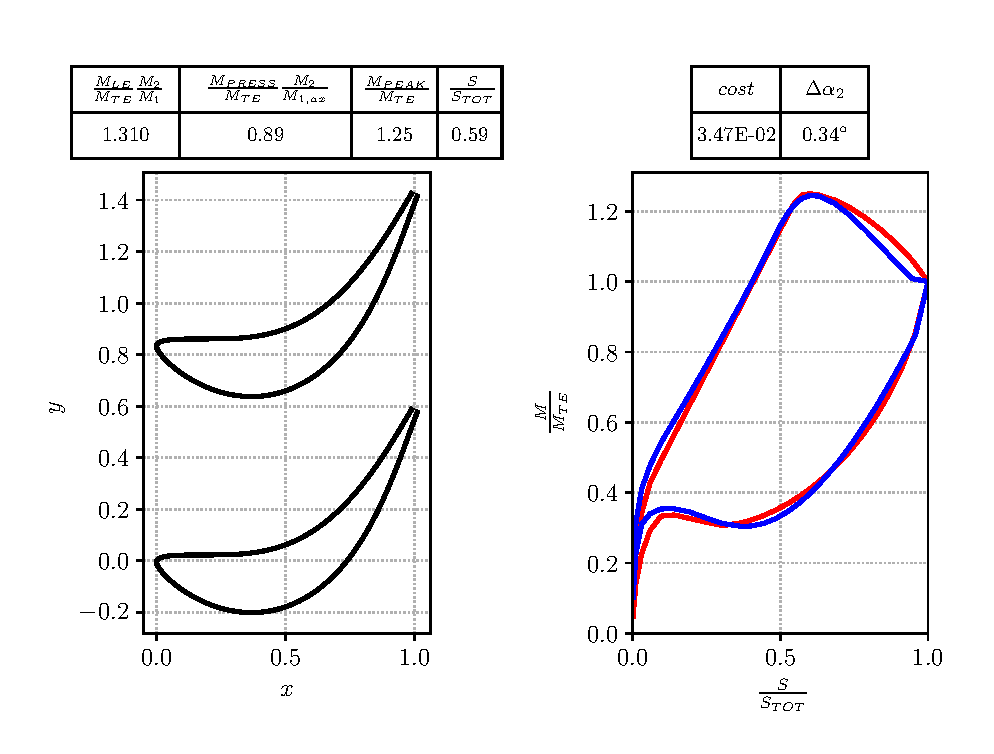
\includegraphics[width=\widthPCA\textwidth]{./images/blade--2007-6516-60.eps}
    \caption{Blade generated by $\hat{\mathnormal{f}}$ with $\alpha_1 = -20.07^{\circ}$, $\alpha_2 = 65.16^{\circ}$ and $M_2 = 0.60$.}
    \label{fig:bladeML4}
\end{figure}

\section{PCA}

% The work introduces the Principal Component Analysis (PCA) as a robust technique for simplifying complex datasets. In this context, PCA operates solely on the $\mathcal{Y}$ dataset.

% PCA initiates with a thorough examination of correlations among various blade parameters:
The work introduces Principal Component Analysis (PCA) as a robust technique for simplifying complex datasets~\cite{geron2022hands}. In this context, PCA operates solely on the $\mathcal{Y}$ dataset.

PCA commences with a comprehensive analysis of correlations among various blade parameters:

\begin{itemize} 
    \item $\gamma$, $\chi_1$, and $\chi_2$ for camberline
    \item $A_{suct}$ for suction-side parametrization
    \item $A_{press}$ for pressure-side parametrization
    \item Pitch
\end{itemize}

% This analysis unearths the principal correlation directions, essentially representing the eigenvectors that define the $\mathcal{Y}$ dataset. Subsequently, the analysis computes additional modal directions, each signifying the dataset's coverage importance, with higher variance equating to broader coverage.

% Notably, the work demonstrate that merely three modes can effectively encompass over $95\%$ of the entire dataset, as evident in Figure~\ref{fig:PCA}.
This analysis uncovers the principal correlation directions, essentially representing the eigenvectors that define the $\mathcal{Y}$ dataset. Subsequently, the analysis computes additional modal directions, each signifying the dataset's coverage importance, with higher variance equating to broader coverage.

Notably, the work demonstrates that only three modes can effectively encompass over $95\%$ of the entire dataset, as evidenced in Figure~\ref{fig:PCA}.

\begin{figure}[!h]
    \centering
    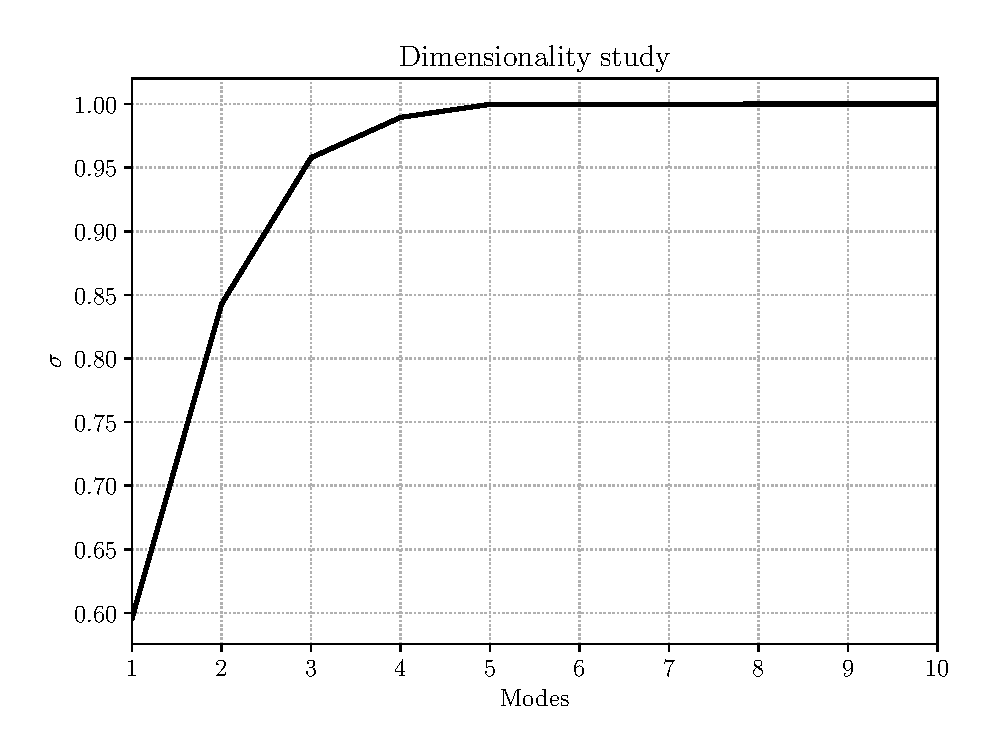
\includegraphics[width=0.5\textwidth]{./images/PCAmodes.eps}
    \caption{Principal Components of $\mathcal{Y}$ dataset.}
    \label{fig:PCA}
\end{figure}

\subsection{Modal Analysis}

% The exploration proceeds with modal analysis, which unveils the significance of each mode within the $\mathcal{Y}$ dataset. Modal analysis further refines the research domain, focusing exclusively on the $\mathcal{Y}$ dataset.

% Figure~\ref{fig:PCAmode1} introduces the first mode, emphasizing its substantial influence on camberline variation and the ensuing suction-side load distribution.
The exploration continues with modal analysis, which reveals the significance of each mode within the $\mathcal{Y}$ dataset. Modal analysis further refines the research domain, concentrating exclusively on the $\mathcal{Y}$ dataset.

Figure~\ref{fig:PCAmode1} introduces the first mode, emphasizing its substantial influence on camberline variation and the resulting suction-side load distribution.

\begin{figure}[!h]
    \centering
    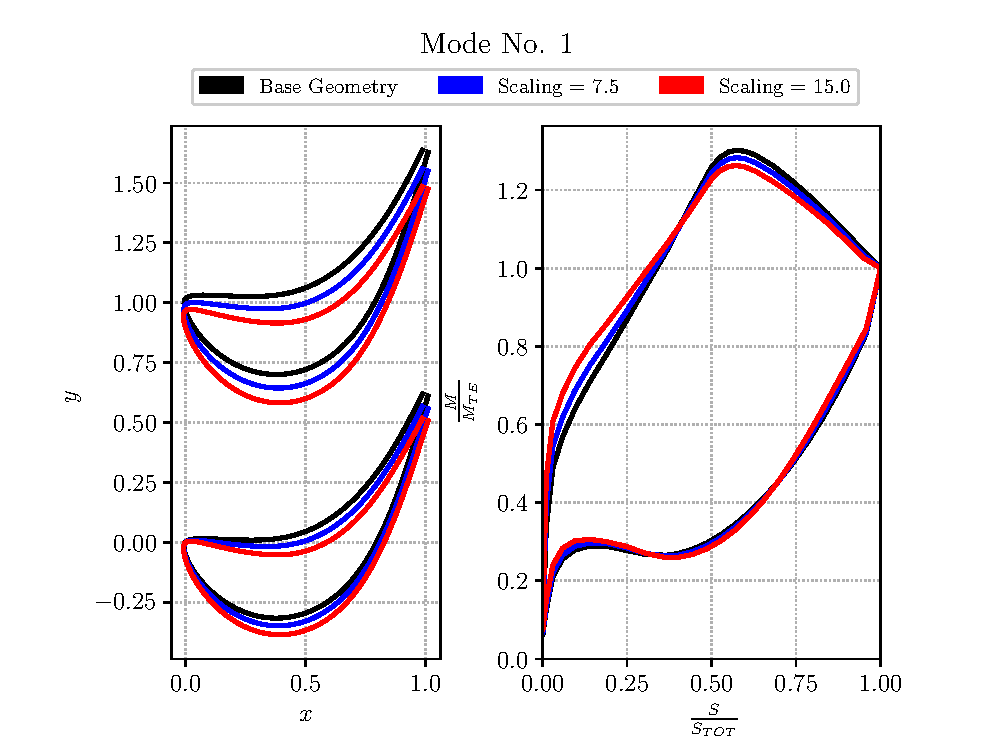
\includegraphics[width=\widthPCA\textwidth]{./images/mode01.eps}
    \caption{Mode No. 1 with the respective modal loading distribution.}
    \label{fig:PCAmode1}
\end{figure}

% Figure~\ref{fig:PCAmode2} delves into the second mode, primarily featuring blade thickness variation and its implications on pressure-side load distribution.

Figure~\ref{fig:PCAmode2} delves into the second mode, primarily highlighting blade thickness variation and its implications on pressure-side load distribution.

\begin{figure}[!h]
    \centering
    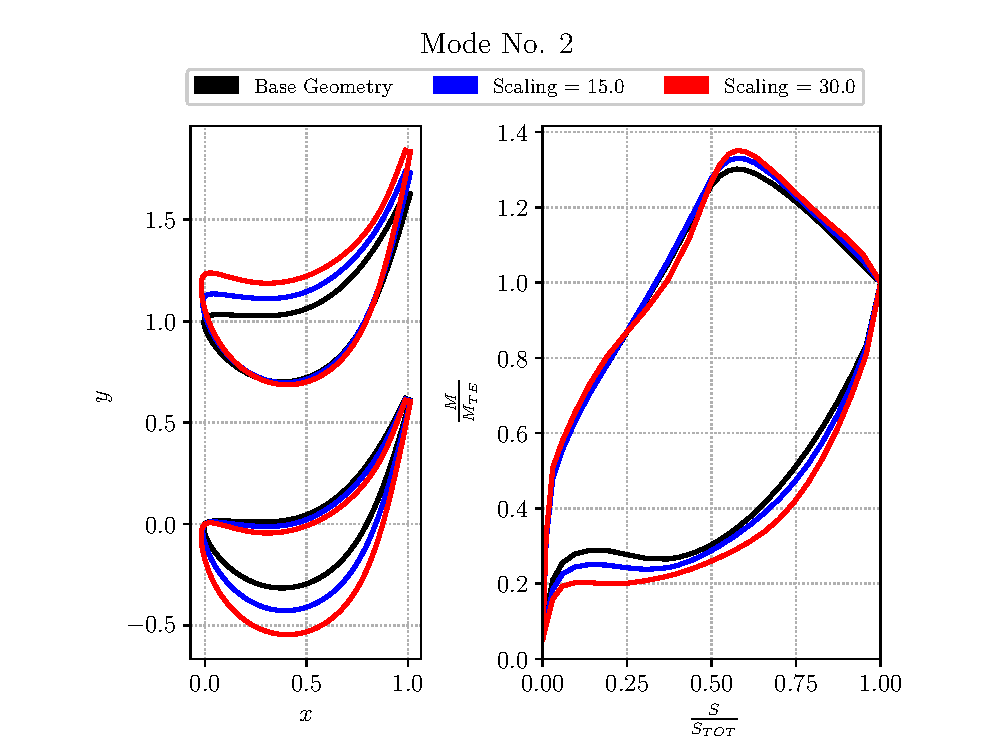
\includegraphics[width=\widthPCA\textwidth]{./images/mode02.eps}
    \caption{Mode No. 2 with the respective modal loading distribution.}
    \label{fig:PCAmode2}
\end{figure}

% Figure~\ref{fig:PCAmode3} unveils the third mode, highlighting changes in the position of the peak Mach number on the suction side and significant alterations in pressure-side Mach distribution.
Figure~\ref{fig:PCAmode3} unveils the third mode, highlighting changes in the position of the peak Mach number on the suction side and significant alterations in pressure-side Mach distribution.

\begin{figure}[!h]
    \centering
    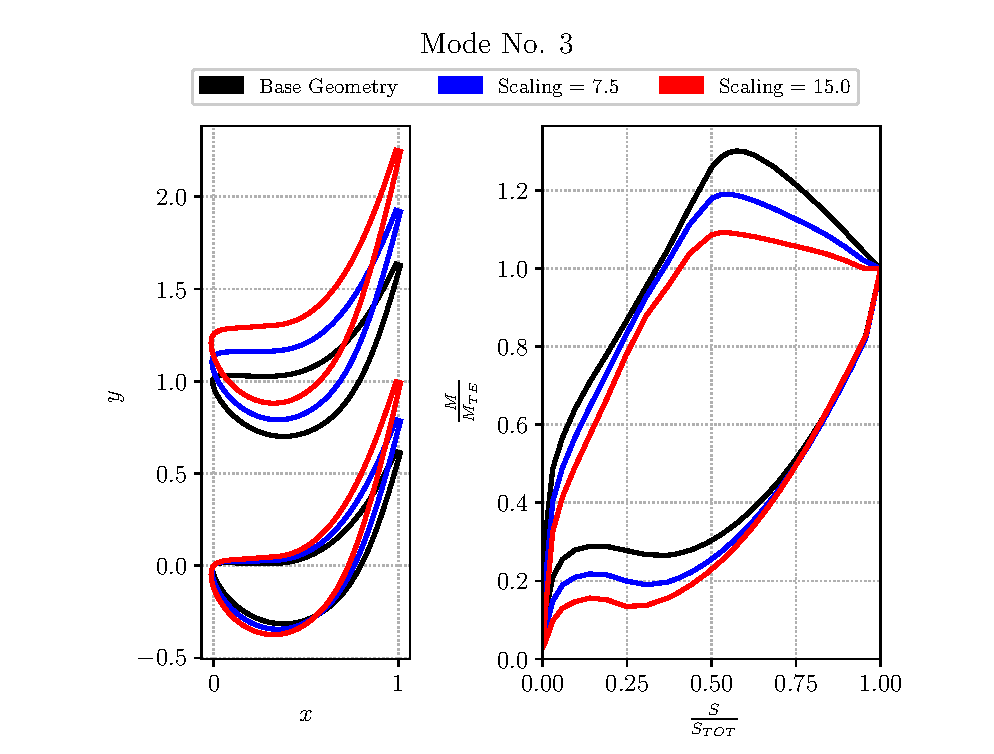
\includegraphics[width=\widthPCA\textwidth]{./images/mode03.eps}
    \caption{Mode No. 3 with the respective modal loading distribution.}
    \label{fig:PCAmode3}
\end{figure} 

% Additionally, the research underscores distinctive modes, including the 10th mode, the 30th mode, and the 42nd mode, each offering unique insights into physical properties.

% Figure~\ref{fig:PCAmode10} elucidates the impact of the 10th mode, primarily affecting pitch and subsequently altering load distribution over the blade.
Additionally, the research emphasizes distinctive modes, including the 10th mode, the 30th mode, and the 42nd mode, each providing unique insights into physical properties.

Figure~\ref{fig:PCAmode10} elucidates the impact of the 10th mode, primarily influencing pitch and subsequently altering load distribution over the blade.

\begin{figure}[!h]
    \centering
    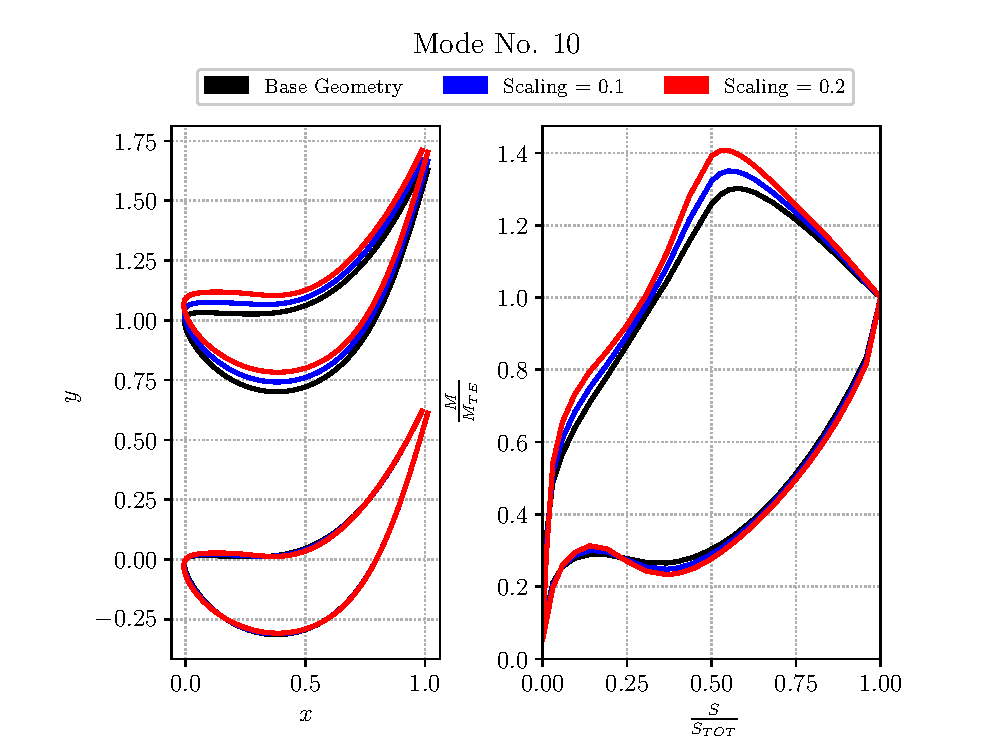
\includegraphics[width=\widthPCA\textwidth]{./images/mode10.eps}
    \caption{Mode No. 10 with the respective modal loading distribution.}
    \label{fig:PCAmode10}
\end{figure}

% Figure~\ref{fig:PCAmode30} illustrates the consequences of a low-variance mode, indicating that avoiding modes with low variance does not significantly compromise geometry representation accuracy.
Figure~\ref{fig:PCAmode30} illustrates the consequences of a low-variance mode, indicating that avoiding modes with low variance does not significantly compromise geometry representation accuracy.

\begin{figure}[!h]
    \centering
    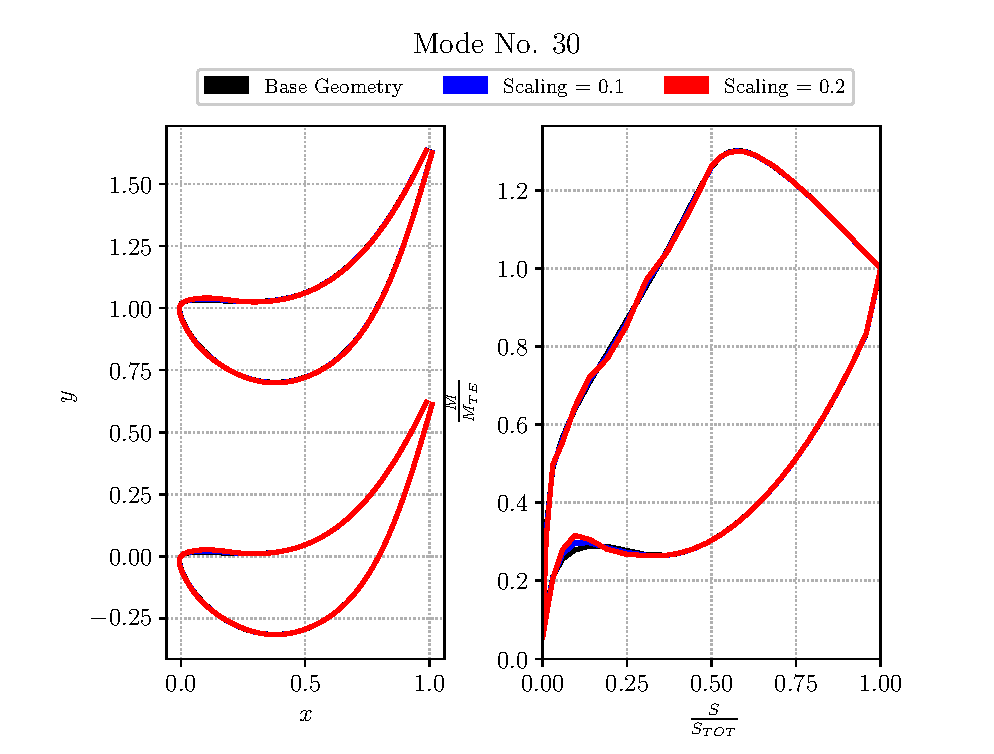
\includegraphics[width=\widthPCA\textwidth]{./images/mode30.eps}
    \caption{Mode No. 30 with the respective modal loading distribution.}
    \label{fig:PCAmode30}
\end{figure}

% Figure~\ref{fig:PCAmode42} introduces the 42nd mode, characterized as a wobbling noise around the blade, emphasizing its minimal importance in blade domain representation.
Figure~\ref{fig:PCAmode42} introduces the 42nd mode, characterized as a wobbling noise around the blade, highlighting its minimal importance in the blade domain representation.

\begin{figure}[!h]
    \centering
    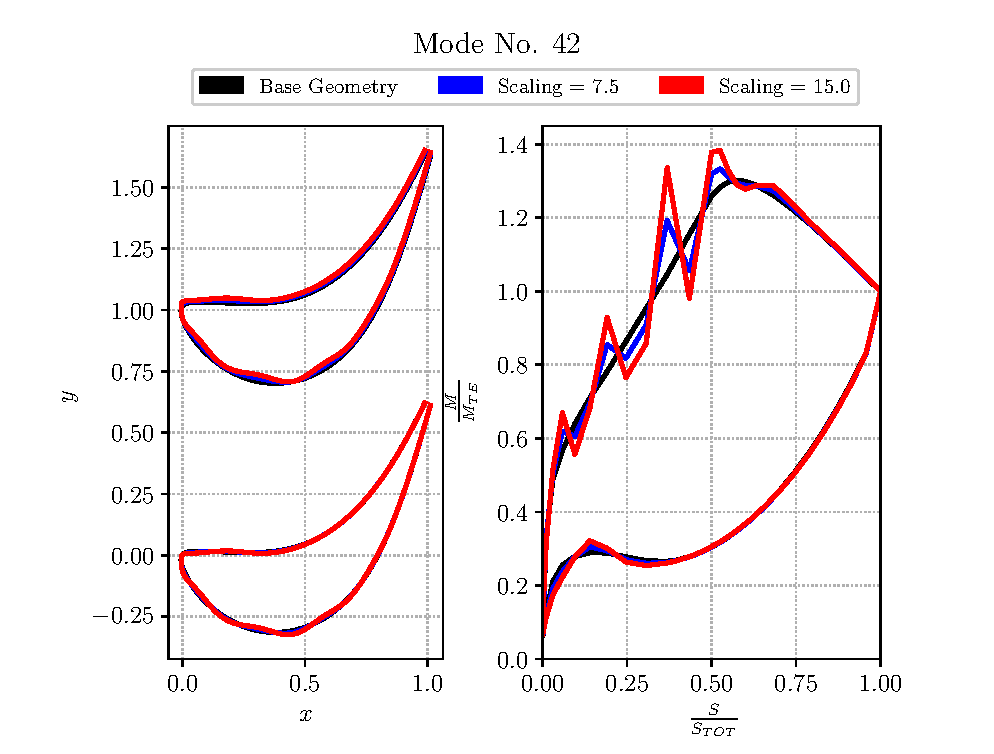
\includegraphics[width=\widthPCA\textwidth]{./images/mode42.eps}
    \caption{Mode No. 42 with the respective modal loading distribution.}
    \label{fig:PCAmode42}
\end{figure}

% \subsection{Synthesis and Recapitulation}

% Chapter 8 marks the culmination of this comprehensive study, encapsulating its main outcomes, limitations, and the prospects of future enhancements.

% \subsection{Innovative Design Paradigm}

% Throughout this research, a groundbreaking design paradigm has been forged for the realm of turbomachinery blade design. This pioneering approach eliminates the conventional reliance on time-consuming Computational Fluid Dynamics (CFD) simulations, ushering in a new era of efficiency. By forging profound correlations between data and blade geometries, it revolutionizes the design process.

\section{Conclusions}

\subsection{Key Insights and Achievements}

% The foremost achievement of this research lies in the successful validation of the proposed methodology. It proves its mettle in blade design, offering speed and the ability to deconstruct the design space into fundamental geometric modes.
The primary achievement of this research lies in the successful validation of the proposed methodology. It demonstrates its effectiveness in blade design, providing both speed and the capability to deconstruct the design space into fundamental geometric modes.

\subsection{Implications and Significance}

% These identified modes hold the promise of crafting blades with enhanced efficiency, leveraging a reduced set of parameters compared to traditional blade parametrization methods. Moreover, by establishing a tangible correlation between blade geometry and parametrized loading distribution, the model empowers designers and imparts a comprehensive understanding of turbomachinery design space and its inherent constraints.
These identified modes hold the promise of crafting blades with enhanced efficiency, utilizing a reduced set of parameters compared to traditional blade parametrization methods. Moreover, by establishing a tangible correlation between blade geometry and parametrized loading distribution, the model empowers designers and imparts a comprehensive understanding of the turbomachinery design space and its inherent constraints.

\subsection{Recognizing Boundaries}

% It is imperative to acknowledge that the model's boundaries are intricately entwined with the laws of physics. The sensitivity of database generation to loading parametrization underscores the model's intimate connection to the realm of physics. Furthermore, the quality of the input database emerges as a pivotal factor that profoundly influences the quality of the resultant blades. Thus, ensuring a high-quality database remains a paramount consideration for optimizing results.
It is imperative to acknowledge that the model's boundaries are intricately entwined with the laws of physics. The sensitivity of database generation to loading parametrization underscores the model's intimate connection to the realm of physics. Furthermore, the quality of the input database emerges as a pivotal factor that profoundly influences the quality of the resultant blades. Thus, ensuring a high-quality database remains a paramount consideration for optimizing results.

\subsection{Forging Pathways Forward}

% Future research endeavors may explore how blade geometry evolves in response to variations in the Reynolds number. Additionally, investigating how blade geometry adapts under diverse loading conditions holds significant promise for advancing this innovative methodology.
Future research endeavors may explore how blade geometry evolves in response to variations in the Reynolds number. Additionally, investigating how blade geometry adapts under diverse loading conditions holds significant promise for advancing this innovative methodology.

\subsection{Concluding Remarks}

% This model's practicality within the industry is manifest, serving as an initial design layer for blade generation. By harmoniously intertwining the realms of physics and machine learning through data integration, it paves the way for a transformative approach to designing turbomachinery systems. This efficient tool streamlines the design process, rendering it accessible to designers from various domains. Its profound significance lies in its ability to reshape the design landscape, ushering in a faster, more intuitive era for turbomachinery system design.
The practicality of this model within the industry is evident, as it serves as an initial design layer for blade generation. By harmoniously intertwining the realms of physics and machine learning through data integration, it paves the way for a transformative approach to designing turbomachinery systems. This efficient tool streamlines the design process, making it accessible to designers from various domains. Its profound significance lies in its ability to reshape the design landscape, ushering in a faster, more intuitive era for turbomachinery system design.

%-----------------------------------------------------------------------------
% HOW TO CITE BIBLIOGRAPHY
%-----------------------------------------------------------------------------
% \nocite{*} % Include all entries from the bibliography database
% \bibliographystyle{plain} % Choose your bibliography style
\bibliographystyle{unsrt}
\bibliography{bibliography.bib} % automatically inserted and ordered with this command 
\label{sec:bibliography}
% The Executive Summary should contain the very essential bibliography of your study.
% It is suggested to use the BibTeX package \cite{bibtex} and save the bibliographic references
% in the file  \verb|bibliography.bib|.

%-----------------------------------------------------------------------------
% CONCLUSION
%-----------------------------------------------------------------------------
% \section{Conclusions}
% A final section containing the main conclusions of your research/study have to be inserted here.

%---------------------------------------------------------------------------
%  ACKNOWLEDGEMENTS 
%---------------------------------------------------------------------------
% \section{Acknowledgements}
% Here you might want to acknowledge someone.

%---------------------------------------------------------------------------
%  BIBLIOGRAPHY
%---------------------------------------------------------------------------
% Remember to insert here only the essential bibliography of your work

\end{document}